\documentclass{beamer}

\usetheme{Madrid}
\usecolortheme{default} % or use {default}

% parse tree
\usepackage[nocenter]{qtree}
\usepackage{tree-dvips}
\usepackage{amsmath}
\usepackage{xcolor}

\usepackage{listings}

\title[]{Semantic Parsing Methods}
\subtitle{An Overview}
\author {Xiang Zhang}
%\institute {
%    NLPR\\
%    Institute of Automation
%}
\date{2016.09.30}
%\logo{\includegraphics[height=1.5cm]{lion-logo.png}}

%------------------------------------------------------------
\AtBeginSection {
    \begin{frame}
        \frametitle{Agenda}
        \tableofcontents[sectionstyle=show/shaded,subsectionstyle=hide/hide/hide]
    \end{frame}
}
\AtBeginSubsection {
    \begin{frame}
        \frametitle{Agenda}
        
        % current subsection / other subsections of current section / other subsections
        \tableofcontents[subsectionstyle=show/shaded/hide]
    \end{frame}
}
%------------------------------------------------------------

\begin{document}

\frame{\titlepage}

%---------------------------------------------------------
%This block of code is for the table of contents after
%the title page
\begin{frame}
\frametitle{Agenda}
\tableofcontents[hideallsubsections]
\end{frame}
%---------------------------------------------------------


\section{Semantics}

\begin{frame}
    \frametitle{Background}

    When it comes to the understanding of natural language sentences, NLP researchers 
    solve it in various granularities.

    These tasks differ in the amount of information they use.

    \begin{itemize}
        \item <1-> Information Extraction (less informative) \\
            \begin{center}
                \emph{is\_a(Obama, PRESIDENT)}
            \end{center}

        \item <2-> Summarization (modestly informative) \\
            \begin{center}
            \emph{Obama wins.}
            \end{center}

        \item <3-> Semantic Parsing (exact matching) \\
            \begin{center}
            $\exists e . beat(e) \wedge Sub(e, Obama) \wedge Obj(e, Romney)$
            \end{center}
            
    \end{itemize}

    \uncover<4->{\begin{block}{Caveat}
        \emph{Semantic} here is more of \emph{composition} than telling apart
        from \emph{word senses}.
    \end{block}}
\end{frame}

\begin{frame}
    \frametitle{Semantic Parsing Task}

    The key task of semantic parsing is to find an $f$ such that

    \[
        f: Sentence \to LogicForm
    \]

    \pause

    Generally, there are 3 aspects a semantic parser need take into consideration:

    \begin{itemize}
        \item Modelling: how to represent a logic form
        \item Parsing: design a grammar and parsing algorithm
        \item Learning: use supervision to fix parameters
    \end{itemize}

\end{frame}


\subsection{Davidsonian Representation}

\begin{frame}
    \frametitle{Logic Form from Example}

    \begin{itemize}

        \item <2->
            Brutus stabs Caesar. \\
            stab(Brutus, Caesar) \structure{predicate}

        \item <3->
            Brutus stabs Caesar with a knife. \\
            stab(Brutus, Caesar, \alert{knife}) \structure{n-ary predicate}

        \item <4->
            Brutus stabs Caesar in the agora. \\
            stab(Brutus, Caesar, \alert{agora}) \structure{ambiguous predicate}

        \item <5->
            Brutus stabs Caesar in the agora with a knife. \\
            stab(Brutus, Caesar) \& \alert{with}(knife) \& \alert{in}(agora)
            \structure{move adjunct apart}

    \end{itemize}

\end{frame}

\begin{frame}
    \frametitle{Logic Form from Example}

    \begin{itemize}
        \item <1-> Brutus stabs Caesar in the agora with a knife. \\
            stab(Brutus, Caesar) \& with(knife) \& in(agora)

        \item <2-> Brutus stabs Caesar with a knife in the agora and twisted it hard. \\
            stab(Brutus, Caesar) \& with(knife) \& in(agora) \& twist(Brutus, knife) \& hard

    \end{itemize}

    \uncover <3-> {
        The standard predicate calculus has problems.

        \begin{itemize}
            \item unable to refer to predicates
            \item natural language are flexible in the number of arguments
                \begin{itemize}
                    \item Pass the axe.
                    \item Pass \alert{me} the axe.
                \end{itemize}
        \end{itemize}
    }

\end{frame}

\begin{frame}
    \frametitle{Davidsonian Representation}

    Semantic is characterized in \emph{events}.
    We don't know an event beforehand, thus we \alert{existentially quantify} it.

    \begin{itemize}

        \item Brutus stabs Caesar with a knife in the agora and twisted it hard.
            \begin{gather*}
                \exists e . stab(e, Brutus, Caesar) \wedge with(e, knife) \wedge in(e, agora)\\
                \wedge (\exists e' . twist(e', Brutus, knife) \wedge hard(e'))
            \end{gather*}

        \item Caesar is stabbed.
            \[
                \exists x \exists e . stab(e, x, Caesar)
            \]

            Missing arguments are left with \alert{placeholders}.
    \end{itemize}

\end{frame}

\begin{frame}

    \frametitle{Problem in Davidsonian Way}

    Consider the following sentence:

    \begin{examples}
        \emph{
            In a dream last night, I was stabbed, although in fact nobody had stabbed me and
            I wasn't stabbed with anything.
        }
    \end{examples}

    There's NOBODY here to initiate the \emph{stab} event.

    The representation should correspond to the \emph{utterance} rather than \emph{reality}?

\end{frame}

\begin{frame}
    \frametitle{neo-Davidsonian Representation (Parson, 1995)}

    Replace \alert{arguments} (and placeholders) with \alert{independent conjuncts}. \pause

    Basically, two roles are important: \alert{Agent}, \alert{Thematic/Patient}. \pause

    \begin{center}
        Brutus stabbed Caesar in the back with a knife
    \end{center}

    \begin{gather*}
        \exists e . stab(e) \wedge Agent(e, Brutus) \wedge Patient(e, Caesar) \\
        \wedge with(e, knife) \wedge in(e, agora)
    \end{gather*}

\end{frame}

\begin{frame}
    \frametitle{Advantages of the neo-Davidsonian (Palmer, 2014)}
    \framesubtitle{(1) Entailment}

    Given the following sentences

    \begin{itemize}
        \item A. Brutus stabbed Caesar
            {\color[rgb]{1,0,0} in the back}
            {\color[rgb]{0,0,1} with a knife}.
        \item B. Brutus stabbed Caesar {\color[rgb]{1,0,0}in the back}.
        \item C. Brutus stabbed Caesar {\color[rgb]{0,0,1}with a knife}.
    \end{itemize}

    We know $A \to B \vee C$ but \alert{NOT} $ B \vee C \to A$.

    \pause

    Using neo-Davidsonian representation preserves this phenomenon.  Let Agt = Agent, B = Brutus, C = Caesar, Pat = Patient, then.

    \begin{itemize}
        \item A. $\exists e . stab(e) \wedge Agt(e, B) \wedge Pat(e, C)
            \wedge in(e, back) \wedge with(e, knife)$

        \item B. $\exists e . stab(e) \wedge Agt(e, B) \wedge Pat(e, C)
            \wedge in(e, back)$

        \item C. $\exists e . stab(e) \wedge Agt(e, B) \wedge Pat(e, C)
            \wedge with(e, knife)$
    \end{itemize}
\end{frame}

\begin{frame}
    \frametitle{Advantages of the neo-Davidsonian}
    \framesubtitle{(2) Scope}

    Traditional way uses scope to connect an adjunct and a verb.

    \begin{center}
        x stabbed y violently with z
    \end{center}

    There're two logically equative representations with different scope settings:

    \begin{itemize}
        \item (with z (violently (stab (y)))) (x)
        \item (violently (with z (stab (y)))) (x)
    \end{itemize}

    But a flat representation like the neo-Davidsonian keeps
    meaning consistent and doesn't introduce explicit syntactic scope.

    {\it The slides will talk about \alert{flat} and \alert{scope} later}.

\end{frame}

\begin{frame}
    \frametitle{Advantages of the neo-Davidsonian}
    \framesubtitle{(3) Temporal and Causal Sentences}

    \begin{itemize}
        \item \emph{Mary saw Brutus stabbed Caesar.}
            \begin{itemize}
                \item Traditional way: \emph{Mary saw Brutus} \& \emph{Brutus stabbed Caesar}.
                \item neo-Davidsonian way \begin{gather*}
                        \exists e . see(e) \wedge Agt(e, Mary) \wedge (
                        \exists e' . stab(e') \wedge Agt(e', Brutus) \\
                        \wedge Pat(e, e')))
                    \end{gather*}
            \end{itemize}

        \item \emph{After the singing of national anthem, they saluted the flag.} \\
            \emph{After the national anthem was sung, they saluted the flag.} \begin{gather*}
                \exists e . salute(e) \wedge Agt(e, they) \wedge Pat(e, flag) \\
                \wedge (\exists e' . sing(e') \wedge Agt(e', they)
                \wedge Pat(e, NationalAnthem) \\
                \wedge after(e, e'))
            \end{gather*}

    \end{itemize}
\end{frame}

\begin{frame}
    \frametitle{Possible Problems of the neo-Davidsonian}

    \begin{itemize}
        \item \emph{I sold him \alert{a car} for \alert{\$50,000}.} \\
            Which is the patient, \emph{car} or \emph{\$50,000}?

            \pause

        \item \emph{I sold a car \alert{for} Mary \alert{for} \$50,000.} \\
            the same preposition with different meanings

            \pause

        \item \emph{Mary fed her baby.} \\
            Can the baby, who is \alert{feeding}, be the agent?

            \pause

        \item \emph{\alert{Brutus} stabbed Caesar \alert{with a knife}.} \\
            The removal of \emph{Brutus} may be different from that of \emph{knife}.

            \pause

        \item \emph{Brutus stabbed Caesar \alert{once}.} \\
            It's hard to specify the event happens only once in neo-Davidsonian.

            \pause

        \item \emph{A saw B leave. When B left, he had the documents in his briefcase.}\\
            $\neq$ \emph{A saw B leave with the documents in his briefcase.} \\
            If both \emph{leave} events are the same, to make the inference work,
            how could A see one one without seeing another?
            
    \end{itemize}
\end{frame}

\begin{frame}
    \frametitle{Summary of the neo-Davidsonian}

    The neo-Davidsonian have several characteristics in representating semantic.
    Some of them are advantages while others are trival choices from various approaches.

    \begin{itemize}
        \item uses variables and is flat.
        \item \alert{event}-style. An event is unique in time of occurrence.
        \item event arguments moved into roles and independent conjuncts.
        \item modifiers(adjectives, adverbs, adjuncts) are conjunct predicates
        \item \emph{transparent} scope
        \item facilitate logical inference
    \end{itemize}

\end{frame}

\subsection{MRS}

\begin{frame}
    \frametitle{Minimal Recursion Semantics (Copestake, 2005)}

    MRS is another \alert{flat} semantic framework,
    serving as the basis of English Resource Semantic (ERS) or English Resource Grammar (ERG).

    \begin{itemize}
        \item Expressive Adequacy: \\
            ability to express meaning correctly
        \item Grammatical Compatibility: \\
            ability to link representations to grammatical information.
        \item Computation Tractability: \\
            ability to compare two representations (equality, relation, etc.)
        \item \alert{underspecifiability}: \\
            leave semantic distinctions unresolved
    \end{itemize}
\end{frame}

\begin{frame}
    \frametitle{An MRS Example}

    \emph{Every big white horse sleeps.}

    \begin{center}
        \Tree [.h0:every(x) {h1:big(x),h1:white(x),h1:horse(x)} h2:sleep(x) ]
    \end{center}
\end{frame}

\begin{frame}
    \frametitle{Why a flat form}

    In MT or other task, a structural representation is hard to use and unnecessary.

    \begin{examples}
        \begin{tabbing}
        Sentence:   \= white English horse \\
        Rule:       \> white(horse)(x) $\leftrightarrow$ Schimmel(x) \\
        Form:  \> white(English(horse)) (x)
        \end{tabbing}
    \end{examples}

    \begin{examples}
        \begin{tabbing}
        Sentence:   \= The beginning of spring arrived. \\
        Rule:       \> beginning of spring $\leftrightarrow$ Fr{\"u}hlingsanfang \\
        Form 1:  \> def\_q(x, spring(x), the(y, beginning(y, x), arrive(y))) \\
        Form 2:  \> the(y, def\_q(x, spring(x), beginning(y, x), arrive(y))) 
        \end{tabbing}
    \end{examples}

\end{frame}

\begin{frame}
    \frametitle{Why a flat form}

    A \emph{flat} form is a group of elementary predicates.

    \begin{examples}
        \begin{tabbing}
        Sentence:   \= white English horse \\
        Rule:       \> white(horse)(x) $\leftrightarrow$ Schimmel(x) \\
        Form:  \> white(x) \& English(x) \& horse(x)
        \end{tabbing}
    \end{examples}

    \begin{examples}
        \begin{tabbing}
        Sentence:   \= The beginning of spring arrived. \\
        Rule:       \> beginning of spring $\leftrightarrow$ Fr{\"u}hlingsanfang \\
        Form:  \> the(y) \& beginning(y, x) \& def(x) \& spring(x) \& arrive(e, y)
        \end{tabbing}
    \end{examples}

\end{frame}

\begin{frame}
    \frametitle{Underspecifiability in MRS}
    There may be several semantically identical representations of a sentence.

    \begin{center}
        \emph{Every dog chases some white cat.}
    \end{center}

    \only<1>{
        \begin{columns}
            \column{0.5\textwidth}

            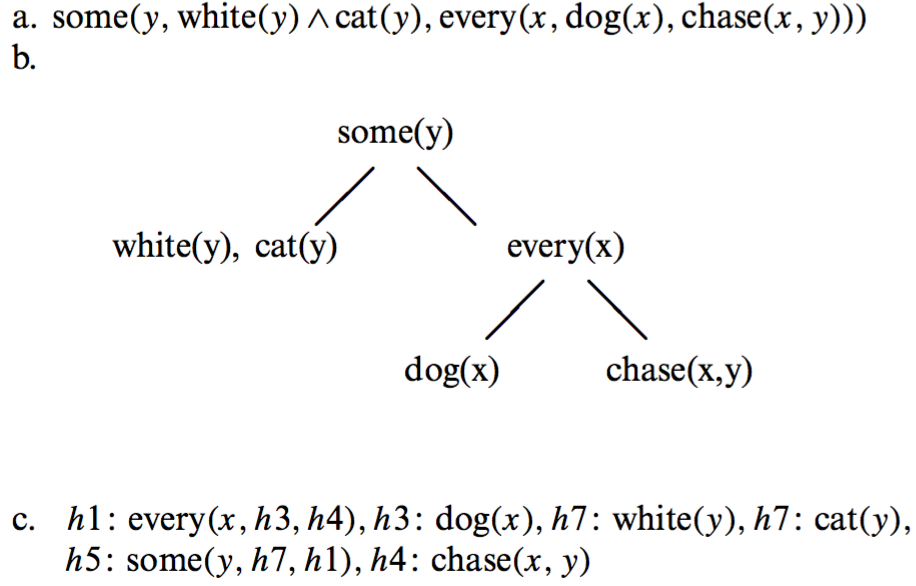
\includegraphics[height=4cm,width=6cm]{img/parse01.png}
            
            \column{0.5\textwidth}
            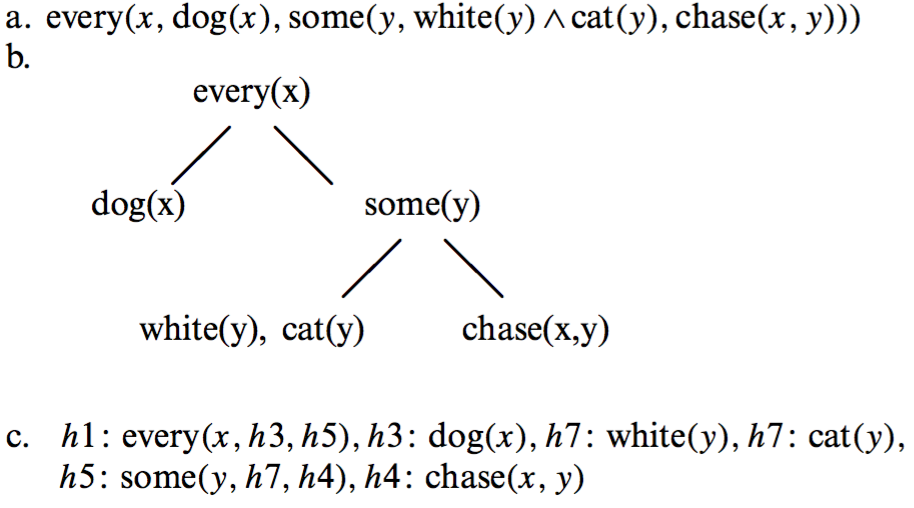
\includegraphics[height=4cm,width=6.3cm]{img/parse02.png}
        \end{columns}
    }

    \only<2>{
        \begin{columns}
            \column{0.7\textwidth}

            Leave some handles unspecified.

            \begin{itemize}

                \item Then specify it later: $h0 = h1, h3 = h5, h7 = h4$

                \item constraints, $h3 \neq h7$ to make it still a tree

                \item qeq constraint, $h0 =_q h5$ is a trival example

            \end{itemize}

            \column{0.3\textwidth}

            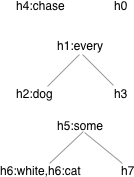
\includegraphics[height=4cm]{img/unresolved-parse.png}

        \end{columns}
    }

\end{frame}

\begin{frame}
    \frametitle{MRS formally in a whole}

    MRS is a quadruple \{GT, LT, R, C\}

    \begin{itemize}
        \item GT: global top. h0
        \item LT: local top. h1, h4, h5 (semantic of local phrase)
        \item R: relations. h1:every(x, h2, h3), h5:dog(y, h6, h7), h4:chase(x), etc.
        \item C: constraints. h0 qeq h4, etc.
    \end{itemize}
\end{frame}

\begin{frame}
    \frametitle{Highlights of MRS}

    \begin{itemize}
        \item We reify scopal relationships as handles
            so that syntactically the language looks first-order.
        \item Preserve \emph{underspecifiability}
    \end{itemize}
\end{frame}

\subsection{AMR}

\begin{frame}
    \frametitle{Abstract Meaning Representation (Banarescu, 2013)}

    AMR is an semantic representation that

    \begin{itemize}
        \item is rooted, directed and labeled graph
        \item is identical for different utterance
        \item uses variables for co-reference
        \item uses PropBank frame (analogous to roles in neo-Davidsonian)
        \item designs non-core relations out of PropBank
            (analogous to adjuncts in neo-Davidsonian)
    \end{itemize}

    Specification: https://github.com/amrisi/amr-guidelines/blob/master/amr.md

\end{frame}

\begin{frame}[fragile] % fragile is for verbatim
    \frametitle{An AMR Example}

    \emph{Brutus stabbed Caesar with a knife in the back in the agora and twisted it hard.}

    \begin{verbatim}
(s / stab
      :ARG0 (p / person :name (n / name :op1 "Brutus")
            :ARG0-of (t / twist
                  :ARG1 k
                  :manner (h / hard)))
      :ARG1 (p2 / person :name (n2 / name :op1 "Caesar"))
      :ARG2 (k / knife)
      :ARG3 (b / back)
      :location (a / agora))
    \end{verbatim}
\end{frame}

\begin{frame}[fragile]
    \frametitle{Event Frames Rise from Various POS}

    \begin{itemize}
        \item Verb \pause
        \item Noun

            \begin{examples}
            \emph{the destruction of the city by the God}
            \begin{verbatim} (d / destroy-01 :ARG0 (g / God) :ARG1 (c / city)) \end{verbatim}
            \end{examples}

            \begin{examples}
            \emph{the bond investor}
            \begin{verbatim} (p / person :ARG0-of (i / invest-01 :ARG1 (b / bond))) \end{verbatim}
            \end{examples}

            \only<2>{but \emph{professor} doesn't yield an event frame}

            \pause

        \item Adjective

            \begin{examples}
            \emph{the attractive spy}
            \begin{verbatim} (s / spy :ARG0-of (a / attract-01)) \end{verbatim}
            \end{examples}
    \end{itemize}
\end{frame}

\begin{frame}[fragile]
    \frametitle{Reification - Frame from Non-Core Relation}

    An adjunct for non-core relation in AMR must serve as a role for the relation,
    rather than for any object participating in that relation.

    \begin{examples}
    \emph{the marble in the jar}
    \begin{verbatim} (m / marble :location (j / jar)) \end{verbatim}

    \emph{the marble is not in the jar}
    \begin{verbatim} (b / be-located-at-91
    :ARG1 (m / marble) :ARG2 (j / jar) :polarity -) \end{verbatim}
    \end{examples}

    \begin{alertblock}{Semantic Error}
    \begin{verbatim} (m / marble :location (j / jar :polarity -)) \end{verbatim}
    which reads \emph{the marble is in the non-jar}
    \end{alertblock}
\end{frame}

\begin{frame}
    \frametitle{Other Language Phenomenons Defined in AMR}

    AMR defines approximately 100 relations for language phenomenons.

    \begin{itemize}
        \item negation and modals
        \item interrogation and wh-questions
        \item named entities
        \item location source, destination, path
        \item cause, concession, condition
        \item quantities, date, time
        \item link with wikipedia article :wiki ``Barack\_Obama''
        \item \dots
    \end{itemize}

\end{frame}

\begin{frame}
    \frametitle{AMR Data Overview}

    1. Annotated Corpus:

    \begin{itemize}
        \item \emph{The Little Prince}, 1274:145:143
        \item \emph{The Little Prince} Chinese Version, 1274:145:143
        \item Bio AMR Corpus from PubMed (cancer) articles, 5452:500:500
        \item LDC Corpus General Release 1.0 (June 2014), 13051 in all, \\
            a new general release is due in summer of 2016
    \end{itemize}

    2. Evaluation: smatch metric, comparison of two AMR

    3. SemEval-2017 Task 9: Parsing and Generation

    \begin{itemize}
        \item English Biomedical Data to AMR (SemEval-2016 Task 8)
        \item AMR to English Generation
    \end{itemize}

    4. A python parser: https://github.com/nschneid/amr-hackathon

\end{frame}
\begin{frame}
    \frametitle{Chinese AMR Corpus Example}

    \begin{center}
        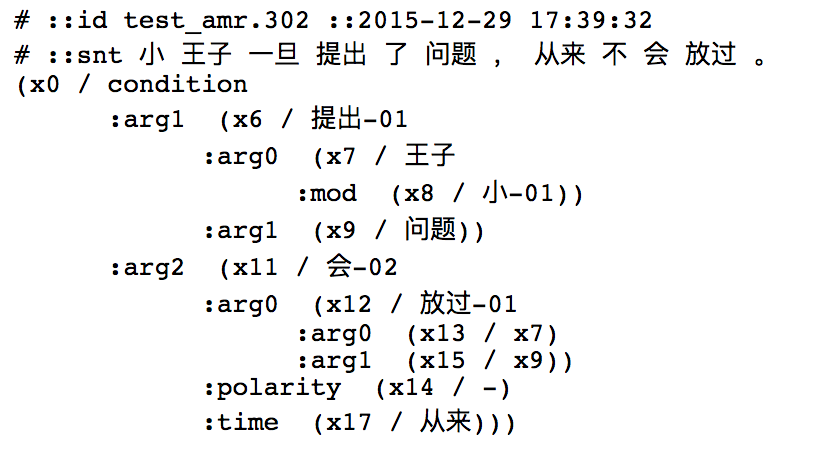
\includegraphics[height=7cm,width=12cm]{img/little-prince-chn-parse.png}
    \end{center}
\end{frame}

\begin{frame}
    \frametitle{AMR Editor}

    A simple web editor to build an AMR.

    \begin{center}
        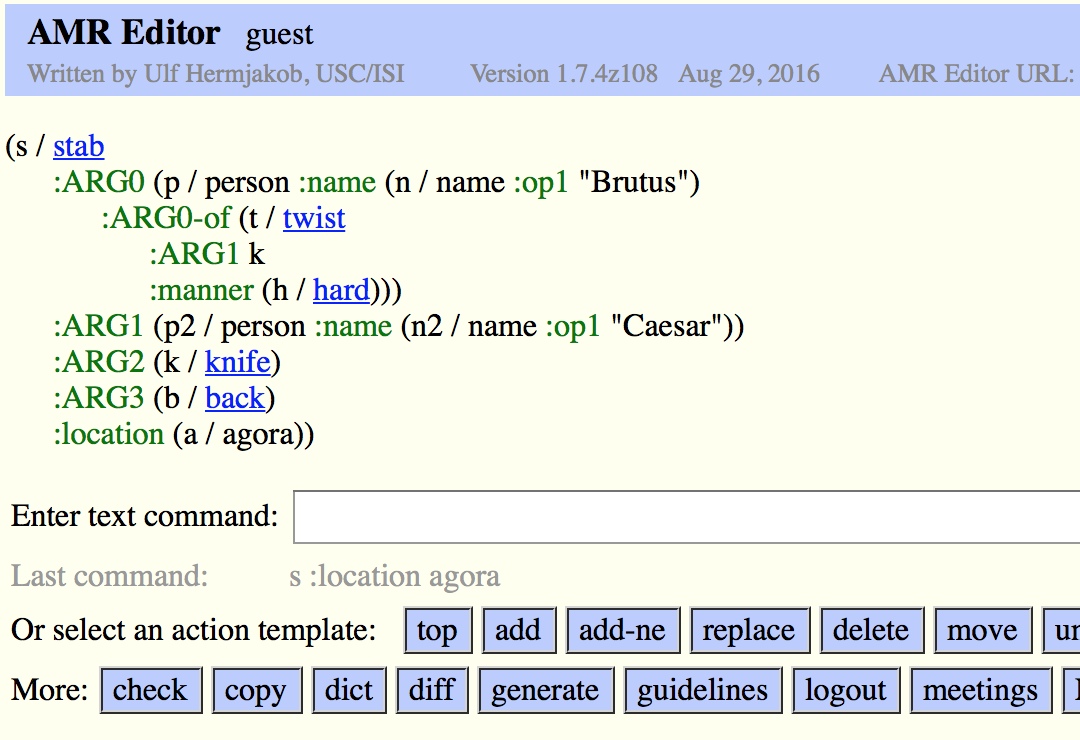
\includegraphics[height=6.7cm,width=9.8cm]{img/amr-editor.png}
    \end{center}
\end{frame}

\section{Parsing}

\begin{frame}
    \frametitle{Parsing Methods}

    There're many semantic parsing paradigms.

    Some of them are new methods while others borrow ideas from other domains or
    tasks to do semantic parsing exactly.

    \begin{itemize}
        \item Shift-Reduce (LR) (1993)
        \item {\bf Combinatory Categorial Grammar (2005)}
        \item {\bf Word Alignment (Synchronized CFG) (2006)}
        \item Generative Model (2008)
        \item {\bf Syntactic Parse to Semantic Parse (2009)}
        \item {\bf Weak Supervision and Unsupervised Methods (2010)}
        \item Large-scale SP for Freebase and QA (2013)
        \item {\bf Paraphrase-driven SP (2014)}
        \item Neural Semantic Parsing (2015)
    \end{itemize}

\end{frame}

\subsection{Shift-Reduce}

\begin{frame}
    \frametitle{Inductive Logic Programming (Zelle et al., 1993)}

    Shift-Reduce is a simple bottom-up parsing. 

    \begin{center}
        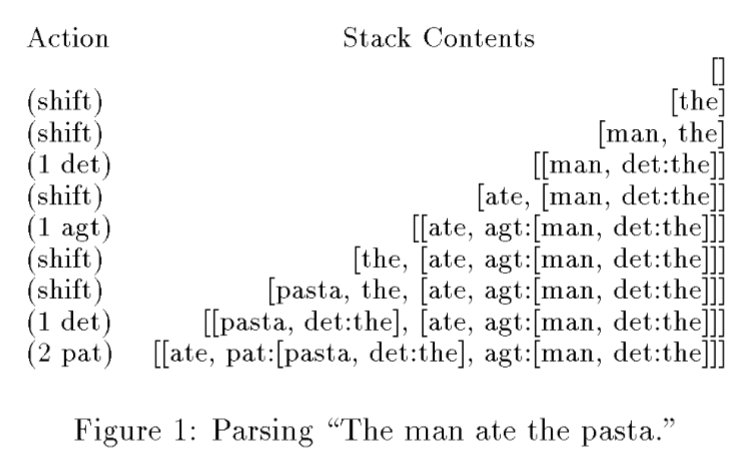
\includegraphics[height=4.62cm,width=7.55cm]{img/shift-reduce.png}
    \end{center}

    Each action correspond to a prolog clause.
    \begin{center}
        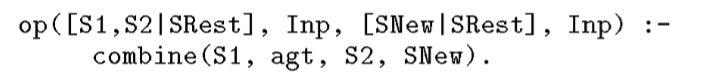
\includegraphics[height=0.6cm,width=6cm]{img/prolog-clause.png}
    \end{center}
\end{frame}

\begin{frame}
    \frametitle{Inductive Logic Programming (Zelle et al., 1993)}

    CHILL(Constructive Heuristic Induction for Language Learning)

    \begin{itemize}
        \item Find\_Generalization: merge clauses not cover any negative sample.
        \item Reduce\_Definition: prefer new clause to prove positive examples
    \end{itemize}

    \begin{center}
        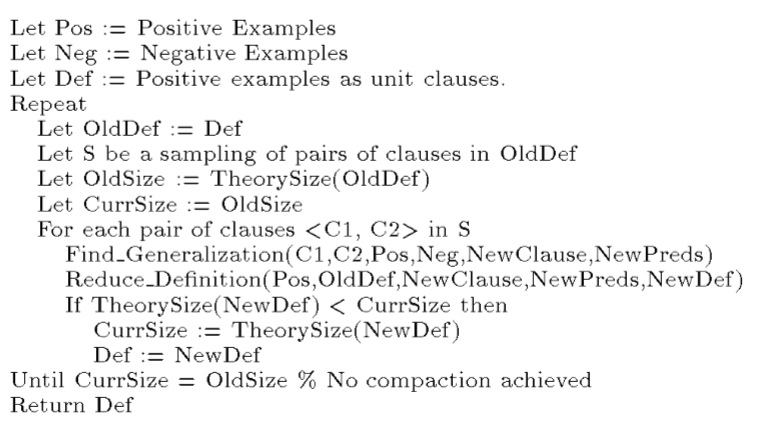
\includegraphics[height=6.5cm,width=10cm]{img/inductive-logic.png}
    \end{center}
\end{frame}

\begin{frame}
    \frametitle{CHILL on GeoQuery (Zelle et al., 1996)}

    \only<1>{
        \begin{columns}
            \column{0.5\textwidth}
            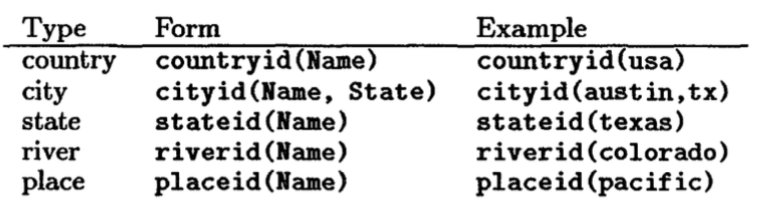
\includegraphics[height=1.7cm,width=5cm]{img/geoquery-object.png}

            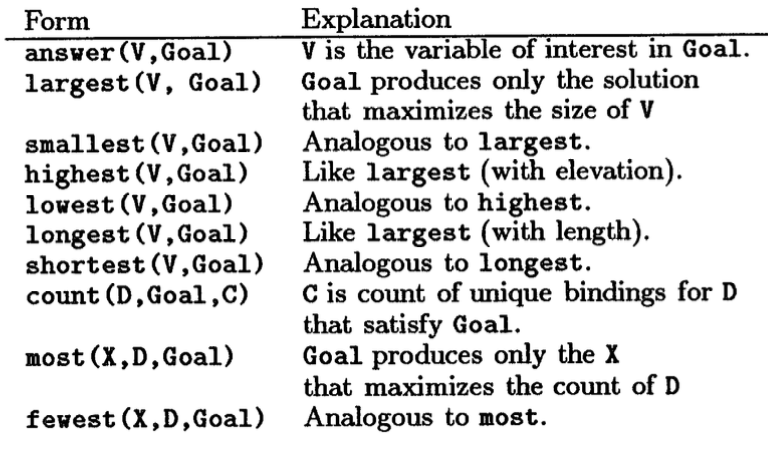
\includegraphics[height=4.5cm,width=6cm]{img/geoquery-meta-predicate.png}

            \column{0.5\textwidth}
            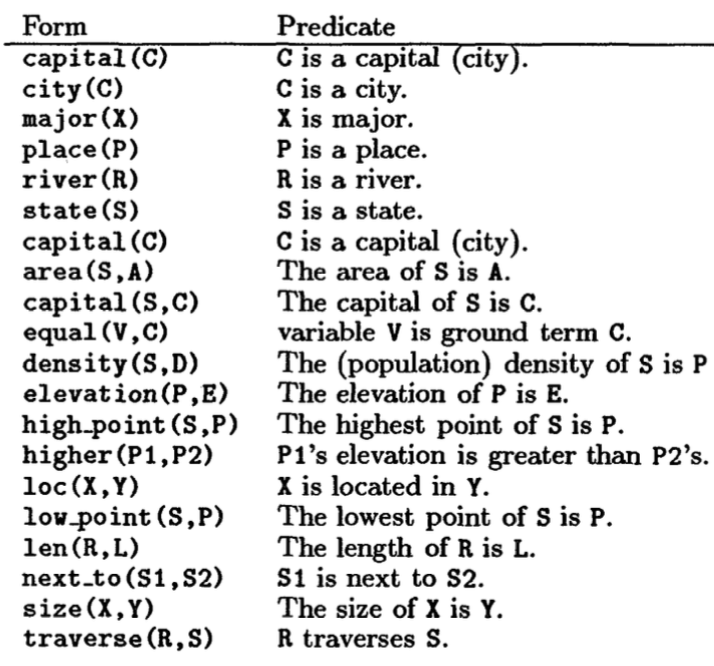
\includegraphics[height=6.5cm,width=6cm]{img/geoquery-predicate.png}
        \end{columns}
    }

    \only<2> {
        \begin{center}
            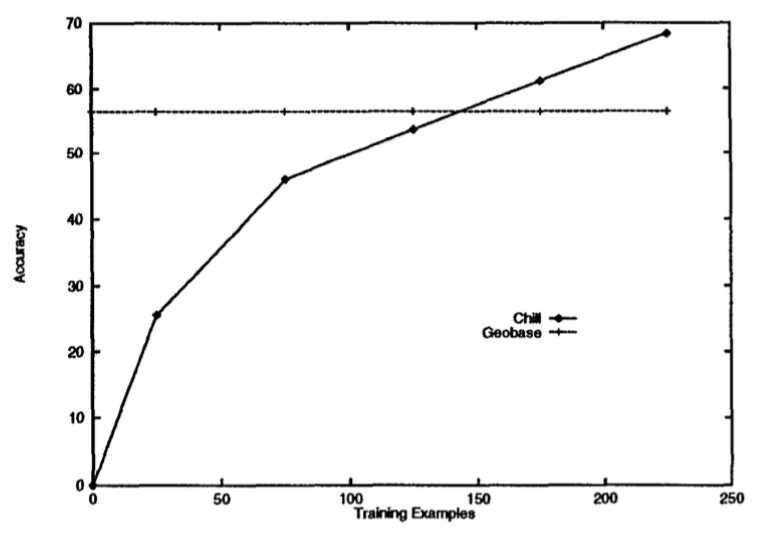
\includegraphics[height=8cm,width=10cm]{img/chill-geoquery-acc.png}
        \end{center}
    }
\end{frame}

\subsection{CCG}

\begin{frame}
    \frametitle{Combinatory Category Grammar (Steedman, 1996, 2000)}

    \only<1> {
        CCG comes with a lexicon whose element is a pair of word and a category:

        \[
            \text{borders} := (S \backslash NP) / NP : \lambda x . \lambda y . borders(y, x)
        \]

        \begin{itemize}
            \item word: $borders$
            \item syntactic type: $(S \backslash NP) / NP$
            \item semantic type: $\lambda x . \lambda y . borders(y, x)$
        \end{itemize}
    }

    \only<2> {
        Categories can be combined.

        \begin{itemize}
            \item forward and backward application

                \begin{tabular}{rlrl}
                    A / B : f &+  &B : x        &$\Rightarrow$ A : f(x) \\
                        B : x &+  &A $\backslash$ B : f &$\Rightarrow$ A : f(x)
                \end{tabular}

            \item forward and backword composition

                \begin{tabular}{rlrl}
                    A / B : f &+  &B / C : g   &$\Rightarrow$ A / C : $f\circ g$  \\
                    A $\backslash$ B : f &+  &B $\backslash$ C : g &$\Rightarrow$
                        A $\backslash$ C : $f\circ g$  \\
                \end{tabular}

            \item type raising

                $X \Rightarrow T / (T \backslash X)$

        \end{itemize}
    }

    \only<3> {
        A CCG Parse Example.

        \begin{center}
            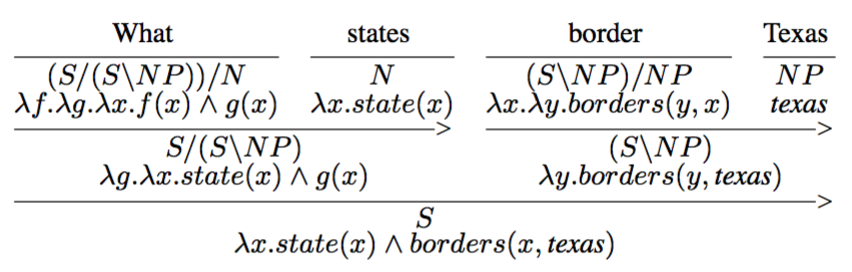
\includegraphics[height=2.72cm,width=8.52cm]{img/ccg-parse.png}
        \end{center}
    }
\end{frame}

\begin{frame}
    \frametitle{Semantic Parsing using CCG on GeoQuery}
    \framesubtitle{Zettlemoyer and Collins, 2005}

    Given the lexicon and model parameter, CCG is formulated as a log-linear probablistic model
    to deal with ambiguity,
    e.g. duplicated lexicon entries for a word, and spurious ambiguity:

    \[
        P(L, T \mid S; \bar\theta) = \frac
            {\exp(\bar f(L,T,S)\cdot\bar\theta)}
            {\sum_{(L,T)}\exp(\bar f(L,T,S)\cdot\bar\theta)}
    \]

    And we can do inference on the model:

    \[
        L = \arg\max_L P(L\mid S;\bar\theta) = \arg\max_L\sum_TP(L,T\mid S;\bar\theta)
    \]

    Features are designed as local and thus we can use dynamic programming
    (beam-search acturally) and prune the search space (like CKY-style).

\end{frame}

\begin{frame}
    \frametitle{Learning the Model (Zettlemoyer et al. 2005)}

    Learning the parameters using SGD.

    \begin{center}
        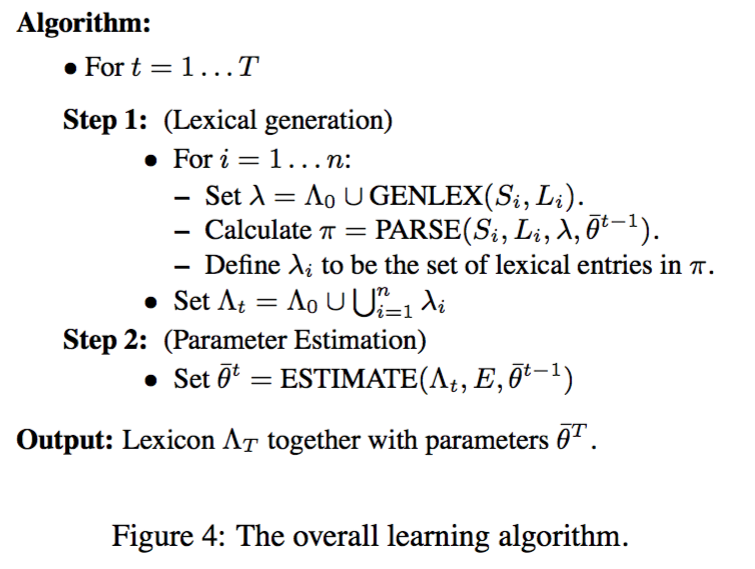
\includegraphics[height=5.69cm,width=7.55cm]{img/learning-algo.png}
    \end{center}

\end{frame}

\begin{frame}
    \frametitle{Learning the Lexicon (Zettlemoyer et al. 2005)}

    \[
        GENLEX(S,L) = \{x := y \mid x \in W(S), y\in C(L)\}
    \]

    \begin{itemize}
        \item W(S) is all subsequence of S
        \item C(L) produces categories using rules L triggered
    \end{itemize}

    \begin{center}
        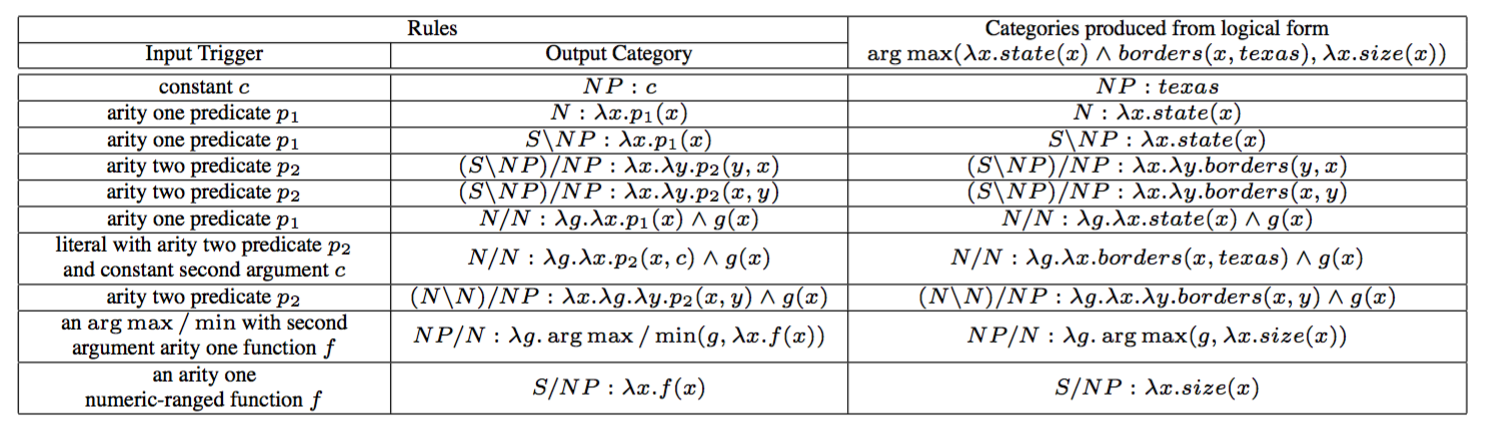
\includegraphics[height=5.32cm,width=12cm]{img/zc05-triggers.png}
    \end{center}

\end{frame}

\begin{frame}
    \frametitle{Problems in ZC05}

    GENLEX is controlled by rules, and will be insufficient
    if the rules don't cover all the (S, L) pairs.

    \begin{examples}
    Through which states does the Mississippi run.
    \end{examples}

    GENLEX doesn't trigger a category suitable for the \emph{through}-adjunct placed ahead.

    Namely, phrase order may be relaxed.
\end{frame}

\begin{frame}
    \frametitle{Relaxed Combinatory Rules (Zettlemoyer et al., 2007)}

    \begin{itemize}
        \item relaxed function application

            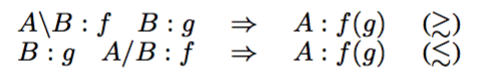
\includegraphics[height=1cm,width=5cm]{img/ccg-relax-01.png}

        \item relaxed function composition

            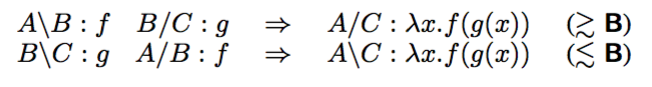
\includegraphics[height=1cm,width=6.5cm]{img/ccg-relax-02.png}

        \item role-hypothesising type shifting (for missing predicates)

            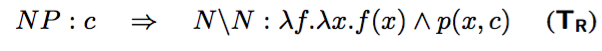
\includegraphics[height=0.6cm,width=6cm]{img/ccg-relax-03.png}

        \item null-head type shifting (for missing arguments)

            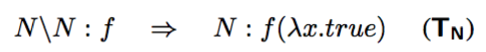
\includegraphics[height=0.6cm,width=5cm]{img/ccg-relax-04.png}

        \item crossed functional composition

            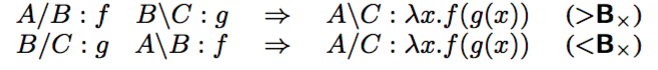
\includegraphics[height=0.8cm,width=6.5cm]{img/ccg-relax-05.png}
    \end{itemize}

    Triggers are added for these new rules, too.

\end{frame}

\begin{frame}
    \frametitle{Online Learning (Zettlemoyer et al., 2007)}

    Use a peceptron learning instead. New features are also added.

    \begin{center}
        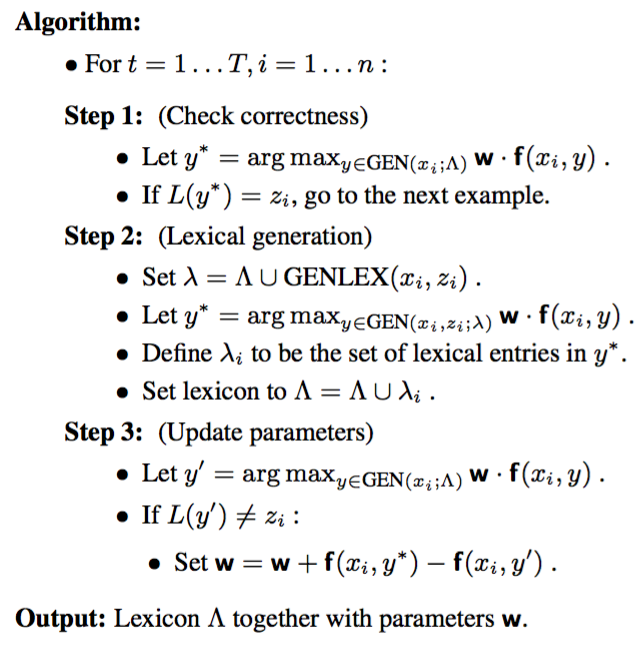
\includegraphics[height=6.5cm,width=6.42cm]{img/zc07-learn-02.png}
    \end{center}
\end{frame}

\begin{frame}
    \frametitle{Problems in ZC07}

    GENLEX needs hand-written rules.
\end{frame}

\begin{frame}
    \frametitle{CCG Induction using Unification (Kwiatkowski et al. 2010)}

    Unification in wikipedia:

    \begin{quotation}
        Unification is an algorithmic process of solving equations between symbolic expressions.
        e.g.
        $\{ cons(x,cons(x,nil)) = cons(2,y) \} \Rightarrow \{  x \to 2, y \to cons(2,nil) \}$
    \end{quotation}

    Here \emph{unification} aims to {\color[rgb]{0,0,1}find f and g given h}, s.t.
    \begin{center}
        $h = \lambda x. f(g(x))$ or $h = f(g)$.
    \end{center} \pause

    For example, the given initial lexical entry
    \[
        \text{New York borders Vermont} \vdash S: next\mathunderscore to(ny, vt)
    \]

    will be splitted as 
    \begin{align*}
        \text{New York borders} &\vdash S / NP : \lambda x . next\_to(ny, vt) \\
        \text{Vermont}          &\vdash NP : vt
    \end{align*}

\end{frame}

\begin{frame}
    \frametitle{CCG Induction using Unification (Kwiatkowski et al. 2010)}

    \only<1> {
        Parsing with PCCG
        \begin{align*}
            P(y, z \mid x; \theta, \Lambda) = \frac{\exp(\theta\cdot\phi(x,y,z))}{Z(y',z')} \\
            f(x) = \arg\max_z p(z\mid x; \theta, \Lambda) \\
            p(z \mid x; \theta, \Lambda) = \sum_y p(y, z \mid x; \theta, \Lambda)
        \end{align*}

        Again, to compute the parse efficiently, 
        \begin{itemize}
            \item CKY-style parsing with dynamic programming
            \item summing over y with inside-outside algorithm
        \end{itemize}
    }

    \only<2> {
        Learning algorithm: NEW-LEX will consider whether to split the lexical entries
        and gives new lexicon from $\arg\max_{y^*}p(y^*\mid x_i, z_i; \theta', \Lambda')$
        \begin{center}
            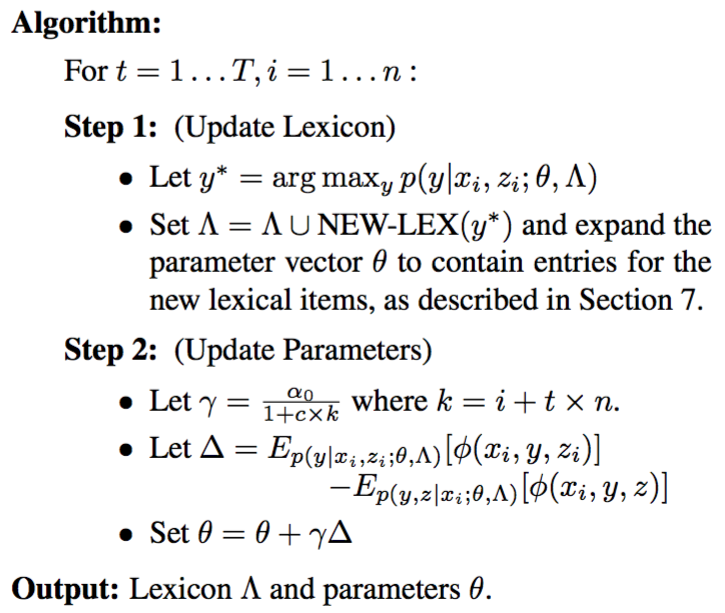
\includegraphics[width=7.25cm,height=6.13cm]{img/unification-learning.png}
        \end{center}
    }

\end{frame}

\begin{frame}
    \frametitle{Split a lexicon (Kwiatkowski et al. 2010)}

    Split a lexical entry: Step 1, function
    \[
        \text{New York borders Vermont} \vdash S: \textcolor{red}{next\_to(ny, vt)}
    \]

    unification constraints (otherwise infinite-result):
    \begin{itemize}
        \item No vacuous variables: $g \ne \lambda x . tex$
        \item limited coordination extraction: $g$ contains less than N adjuncts
        \item limited application: $f$ contains no new variables for non-variable
            subexpression in $h$ like 
            \begin{align*}
                h &= \lambda x . in(x, tex) \\
                f &\to \lambda q . q(tex) \\
                g &\to \lambda y \lambda x . in(x, y)
            \end{align*}
    \end{itemize}

    \pause

    we can get many (f, g) pairs, among which there is: 
    \[
        f \to \lambda x . next\_to(ny, x)\,\,\,\,\, g \to vt
    \]
\end{frame}

\begin{frame}
    \frametitle{Split a lexicon (Kwiatkowski et al. 2010)}

    Split a lexical entry: Step 2, syntactic type
    \[
        \text{New York borders Vermont} \vdash \textcolor{red}{S}: next\_to(ny, vt)
    \]

    \only<1> {
        According to CCG combinatory rules(only 4 here), define
        \begin{align*}
            S_C(A) &= \{FA(A) \cup BA(A) \cup FC(A) \cup BC(A) \}\\
            FA(X:h)&= \{ (X / Y : f, Y : g) \mid h = f(g) \wedge Y = C(T(g)) \}  \\
            BA(X:h)&= \{ (Y : g, X \backslash Y : f) \mid h = f(g) \wedge Y = C(T(g)) \}  \\
            FC(X / Y:h)&= \{ (X / W : f, W / Y : g) \mid
                h = \lambda x . f(g(x)) \wedge W = C(T(g(x))) \}  \\
            BC(X \backslash Y:h)&= \{ (W \backslash Y : f, X \backslash W : g) \mid
                h = \lambda x . f(g(x)) \wedge W = C(T(g(x))) \}
        \end{align*}
        where $T: F \to \{e, t, F\}$ is the type function and C is defined as
        \begin{gather*}
            C(T) = \begin{cases}
                NP & \text{ if } T=e \\ 
                S & \text{ if } T=t \\ 
                C(T_2)\vert C(T_1)  & \text{ if } T= \langle T_1, T_2\rangle
            \end{cases}
        \end{gather*}
    }

    \only<2> {
        These are some possible pair from the splitting set.
        \begin{itemize}
            \item Semantic: \textcolor{blue}{$(\lambda x . next\_to(ny, x), vt)$}

                Syntactic: $(S/NP, NP)$

            \item Semantic: \textcolor{blue}{$(ny, \lambda x . next\_to(x, vt))$}

                Syntactic: $(NP, S\backslash NP)$

            \item Semantic: \textcolor{red}{$(\lambda x . next\_to(x, vt), ny)$}

                Syntactic: $(S/NP, NP)$

        \end{itemize}
    }

\end{frame}

\begin{frame}
    \frametitle{Split a lexicon (Kwiatkowski et al. 2010)}

    Split a lexical entry: Step 3, word sequence
    \[
        \textcolor{red}{\text{New York borders Vermont}} \vdash S: next\_to(ny, vt)
    \]
    Splitting is defined as
    \[
        S_L(w_{0:n}\vdash A) = \{(w_{0:i}\vdash B, w_{i+1:n}\vdash C) \mid
            0 \leq i < n \wedge (B, C) \in S_C(A) \}
    \] \pause
    For some specific i, the previous splits may raise problems.
    \begin{itemize}
        \item \textcolor{blue}{$(S/NP:\lambda x . next\_to(ny, x), NP:vt)$}

            Sequence: (New York borders, Vermont)

        \item \textcolor{blue}{$(NP:ny, S\backslash NP:\lambda x . next\_to(x, vt))$}

            Sequence: (New York, borders Vermont)

        \item \textcolor{red}{$(S/NP:\lambda x . next\_to(x, vt), NP:ny)$}

            Sequence: (borders Vermont, New York) incorrect

    \end{itemize}

\end{frame}

\begin{frame}
    \frametitle{Problems in Kwiatkowski et al. 2010}

    Learned CCG lexicon is too big.
\end{frame}

\begin{frame}
    \frametitle{Factored Lexicon in CCG (Kwiatkowski et al 2011)}

    Original lexical entry: $Boston \vdash N / N:\lambda f\lambda x.from(x, bos) \wedge f(x)$

    Factored Parts:
    \begin{itemize}
        \item lexeme, pair of a word span and a constant list: $(Boston,[from,bos])$
        \item template, $\lambda (w, \vec v).(w \vdash N / N:\lambda f\lambda x.v_1(x, v_2) \wedge f(x))$
    \end{itemize}

    \pause

    Two type of factorization:
    \begin{enumerate}
        \item maximal factor: all constants are in lexeme

            $(Boston, [from, bos]),  
            \lambda (w, \vec v).(w \vdash N / N:\lambda f\lambda x.v_1(x, v_2) \wedge f(x))$

        \item partial factor: some constants remain in the template
            $(Boston, [bos]), 
            \lambda (w, \vec v).(w \vdash N / N:\lambda f\lambda x.from(x, v_1) \wedge f(x))$

            Partial factor is used for missing words: \emph{flights Boston to New York}
    \end{enumerate}

\end{frame}

\begin{frame}
    \frametitle{Factored Lexicon in CCG (Kwiatkowski et al 2011)}

    Learning is similar but to consider factorization:

    \begin{center}
        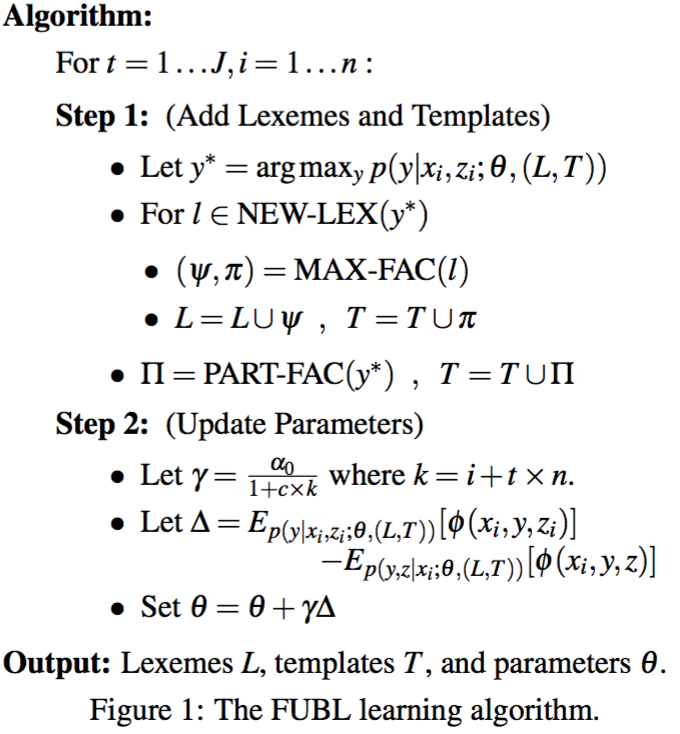
\includegraphics[width=6.8cm,height=7.34cm]{img/fubl.png}
    \end{center}

\end{frame}

\begin{frame}
    \frametitle{Ontological Mismatch Problem}

    GeoQuery / ATIS dataset is too small. Learning a parser is easy for it.
    \begin{itemize}
        \item a few predicates
        \item a few utterances (more than predicate)
    \end{itemize} \pause

    If a database has more predicates and thus more capable to answer more questions
    in theory, the amount of possible utterance can go even further. \pause

    What's worse, new utterances linguistically involve more predicates in theory,
    but database schema is fixed and supports only limited predicates. \pause

    \begin{itemize}
        \item parse to more predicates: unusable on databases
        \item parse to fit the schema: difficult to learn
    \end{itemize}

\end{frame}

\begin{frame}
    \frametitle{SP with On-the-fly Matching(Kwiatkowski et al., 2013)}

    \begin{center}
        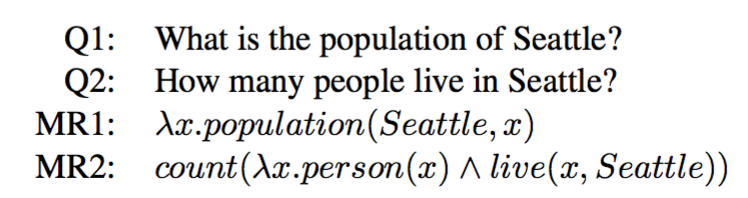
\includegraphics[width=7.48cm,height=1.98cm]{img/ontological-mismatch.png}
    \end{center}

    Choose to convert Q1 to MR1, Q2 to MR2, then MR2 to MR1. Using Q-A pairs.
\end{frame}

\begin{frame}
    \frametitle{SP with On-the-fly Matching(Kwiatkowski et al., 2013)}

    \only<1> {
        Parsing Framework
        \begin{itemize}
            \item Domain-independent parsing
                
                use a domain-independent CCG parser(Clark \& Curran, 2007) to convert 
                the utterance to {\bf underspecified LF}, with a hand-written lexicon
                \begin{itemize}
                    \item 59 lexical categories with POS tags, and assign to words based on POS 
                        tags from Wiktionary.
                    \item 49 domain-independent lexical items (what, when, and, is, etc.)
                \end{itemize}

            \item Ontological Matching
                
                Use a series of matching operations $M = \langle o_1, o_2, \cdots \rangle$
                \begin{itemize}
                    \item Structural Match: Collapse Operator, Expansion Operator
                    \item Constant Matching (replace in the same type)
                \end{itemize}

        \end{itemize}
    }

    \only<2> {
        \begin{center}
            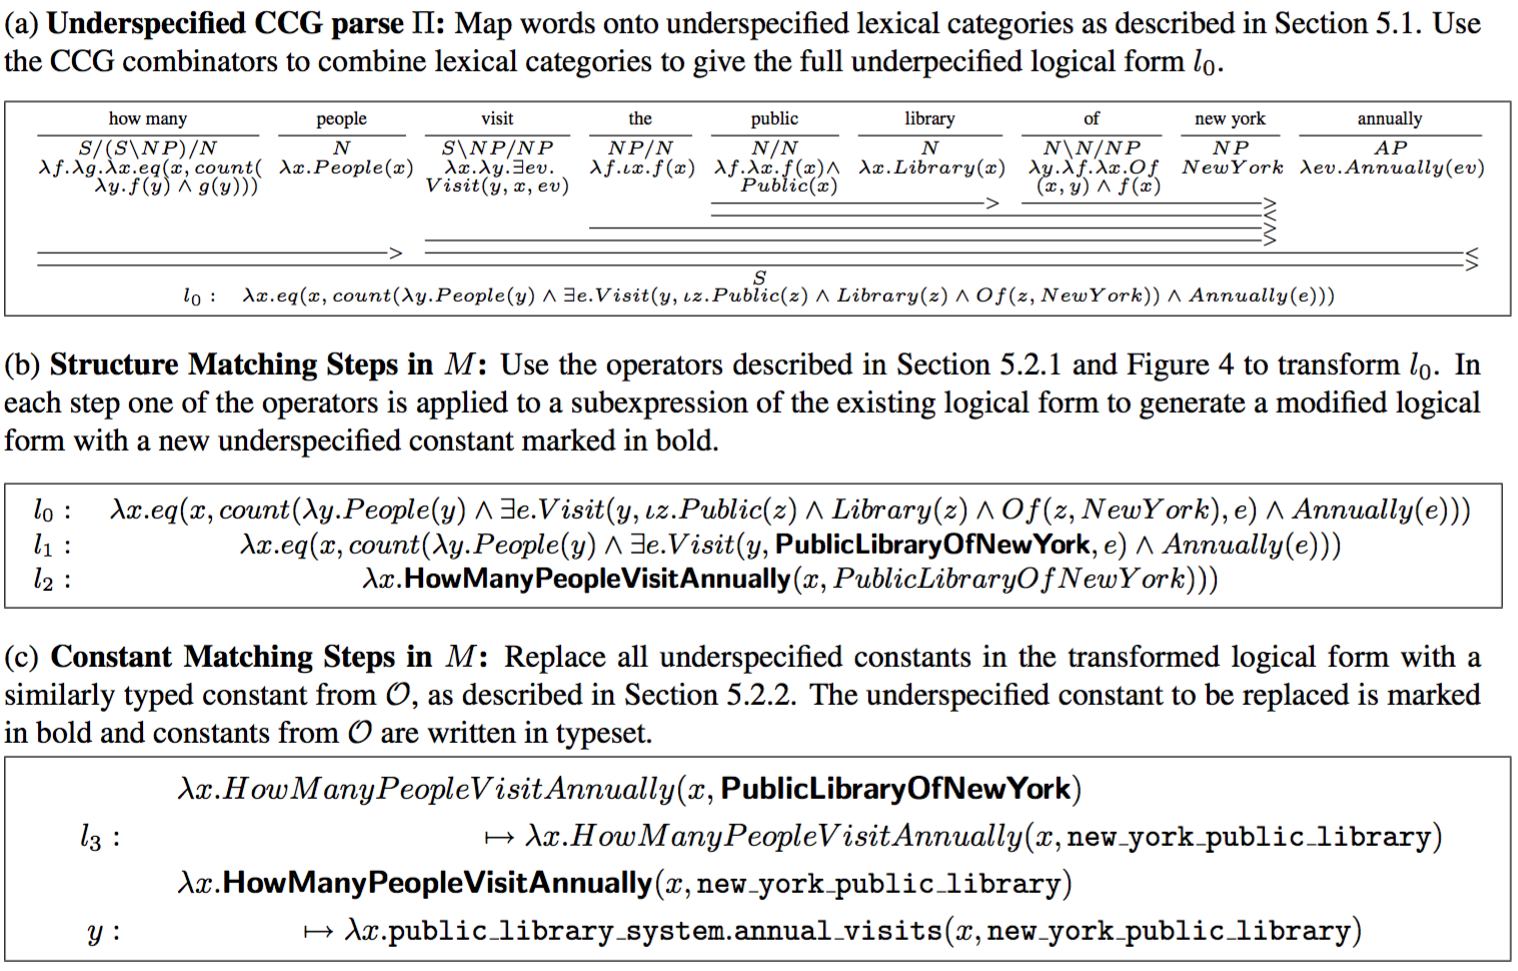
\includegraphics[width=11.5cm,height=7cm]{img/ccg-fb-parse.png}
        \end{center}
    }

    \only<3> {
        \begin{center}
            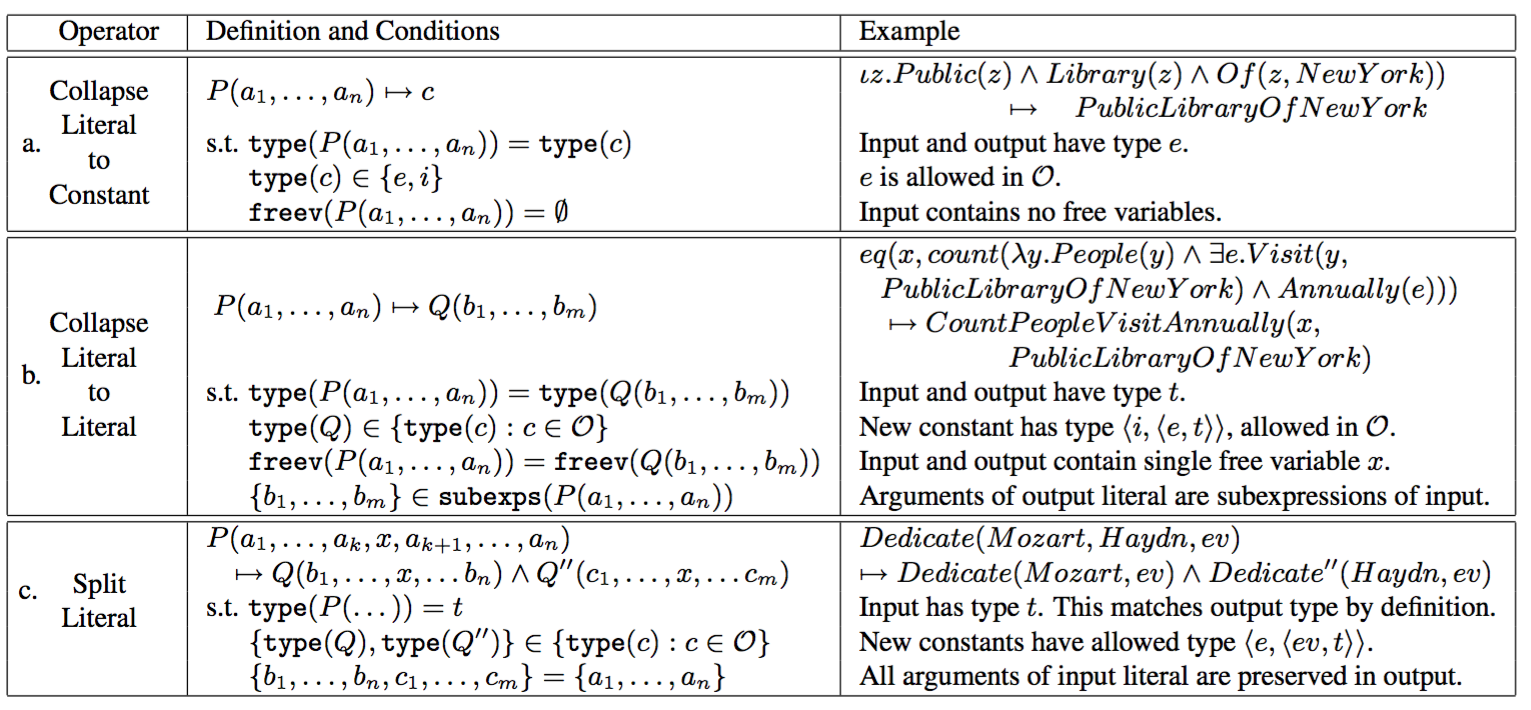
\includegraphics[width=12cm,height=7cm]{img/ontology-match-ops.png}
        \end{center}
    }

    \only<4> {
        Parsing and Learning:
        \begin{align*}
            Parse(x, O) &= {\arg \max}_{d\in GEN(x,O)} (Score(d)) \\
            Score(d)  &= \phi(d) \theta \\
            &= \phi(\Pi)\theta + \sum_{o\in M}\phi(o)\theta
        \end{align*}
        \begin{center}
            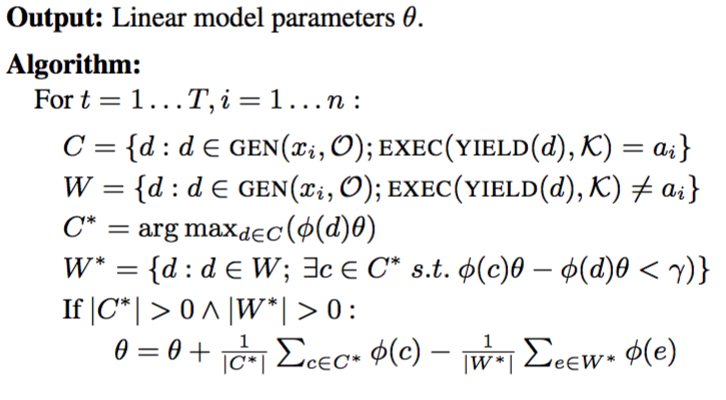
\includegraphics[width=7.26cm,height=4cm]{img/ccg-fb-learning.png}
        \end{center}
    }

    \only<5> {
        Features:
        \begin{itemize}
            \item CCG Parse Features(Pi): \#u\_category, \#(word, category), \#(POS, category)
            \item Structural Features(M): identity of complex-typed const., domain-indep. const.
            \item Lexical Features(M): for $(c_u, c_O)$, $\phi_{np}$, $\phi_{stem}$,
                $\phi_{syn}$, $\phi_{fp:stem}$, $\phi_{def\_overlap}$

            \item Knowledge Base Features: exec y on K, $\phi_{direct}$, $\phi_{join}$,
                $\phi_{empty}$, $\phi_0$, $\phi_1$
        \end{itemize}
    }
\end{frame}

\begin{frame}
    \frametitle{Other CCG Works}
    \begin{itemize}
        \item Artzi et al., TACL2013, Weakly Supervised Learning of Semantic Parsers
            for Mapping Instructions to Actions

            Modeling robot instruction and get feedback from robot action.

        \item Reddy et al., TACL2014, Large-scale Semantic Parsing without Question-Answer Pairs

            Use ClueWeb09 and FACC1, and general CCG parser to build a LF,
            which is then converted to an ungrounded graph sharing commonalities with Freebase.

        \item Artzi et al., EMNLP2015, Broad-coverage CCG Semantic Parsing with AMR

            To deal with co-reference in AMR, use Skolem Terms (Steedman, 2011) to build
            an underspecified LF, which is then mapped to specified LF.

    \end{itemize}
\end{frame}

\subsection{Word Alignments}

\begin{frame}
    \frametitle{Learning SP with SMT(Wong and Mooney, 2006)}
    \only<1> {
        Synchronized CFG rule: $X \to \langle \alpha, \beta \rangle$
        (pattern \& template)
        \begin{center}
            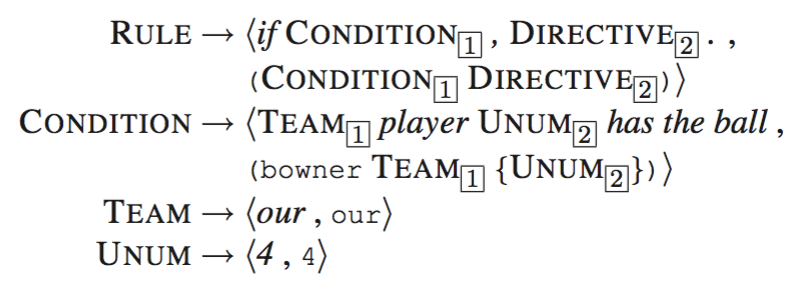
\includegraphics[width=7.88cm,height=2.94cm]{img/scfg-rule.png}

            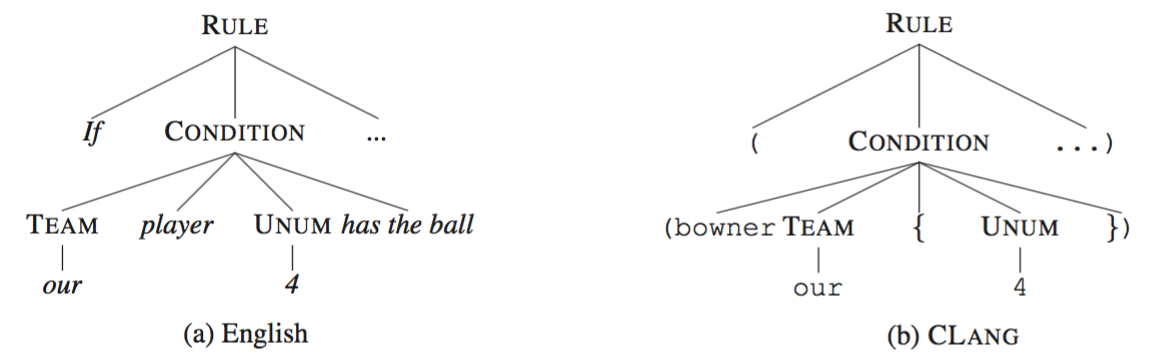
\includegraphics[width=11.74cm,height=3.64cm]{img/scfg-parse.png}
        \end{center}
    }

    \only<2> {
        Parsing: enumerate derivations that gives $\langle e, f \rangle$
        \begin{align*}
            f^* &= m(\arg\max_{\mathrm{d}\in D(G\mid e)}\Pr(\mathrm{d}\mid e; \lambda)) \\
            \Pr_\lambda(d\mid e) &= \frac{1}{Z_\lambda(e)}\exp\sum_i\lambda_i f_i(d)
        \end{align*}
        Features (3000 or so):
        \begin{itemize}
            \item number of each rule r is used in derivation
            \item number of each word w generated from gaps
        \end{itemize}

        Parameter Estimation: 

        Viterbi algorithm is used for efficient decoding.

        Since gold derivation is latent, EM is used to find the optimal parameters.
    }

\end{frame}

\begin{frame}
    \frametitle{Learning SP with SMT(Wong and Mooney, 2006)}

    Grammar rules acquisition:

    \only<1> {
        Step 1, suppose we know the grammar, LF can be convert to a production (rule) sequence
        of the left-most top-down derivation (by convention).

        We prefer derivation sequence over LF because MR may be not well-formed
        without grammar and MR tokens can be polysemy or carry no specific meaning.

        \begin{examples}[Sentence and LF from RoboCup]
            ((bowner our \{4\}) \\
            (do our \{6\} (pos (left (half our))))) \\
            If our player 4 has the ball, \\
            then our player 6 should stay in the left side of our half.
        \end{examples}
    }

    \only<2>{
        Step 2, use GIZA++ to find alignment between words and derivation rules.

        \begin{center}
            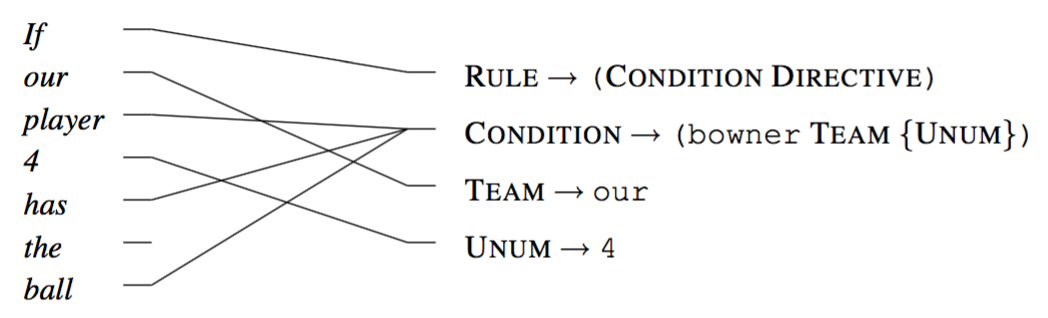
\includegraphics[width=10.48cm,height=3.18cm]{img/wong-align.png}
        \end{center}
    }

    \only<3> {
        Step 3, extract bottom up, starting with rules where RHS contains only terminals,
        then those whose RHS contains non-terminals.
        \begin{center}
            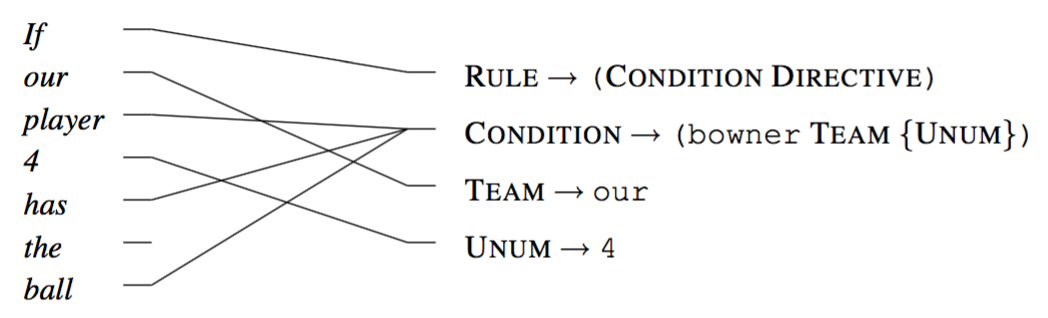
\includegraphics[width=10.48cm,height=3.18cm]{img/wong-align.png}
        \end{center}
        \begin{align*}
            UNUM &\to \langle 4, 4 \rangle \\
            TEAM &\to \langle our, our \rangle \\
            CONTITION &\to \langle TEAM \text{ player } UNUM \text{ has \{1\} ball }, \\
                & (bowner\, TEAM\, \{UNUM\})\rangle
        \end{align*}
    }

    \only<4> {
        Step 3 special case: rule that doesn't derive any terminal, and that break links
        outside this sub-parse tree.
        \begin{center}
            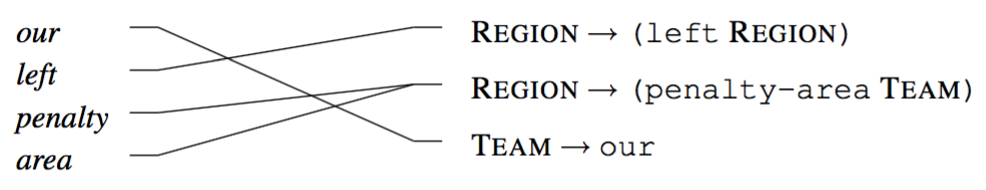
\includegraphics[width=9.86cm,height=1.9cm]{img/phrasal-coherence.png}
        \end{center}

        Merge the rules as: $REGION \to (\text{left } (\text{penalty-area } TEAM)$

        For excessively merged rules (overfitting), try a greedy link-removal policy
        (alignment fixing).
    }
\end{frame}

\begin{frame}
    \frametitle{SCFG with Lambda Calculus(Wong and Mooney, 2007)}
    Use lambda expression for semantic function instead. To improve NL-MR isomorphism,
    find a MST on a graph where edges between rules are established for any shared variable and 
    weighted by the minimal word distance.
    \begin{center}
        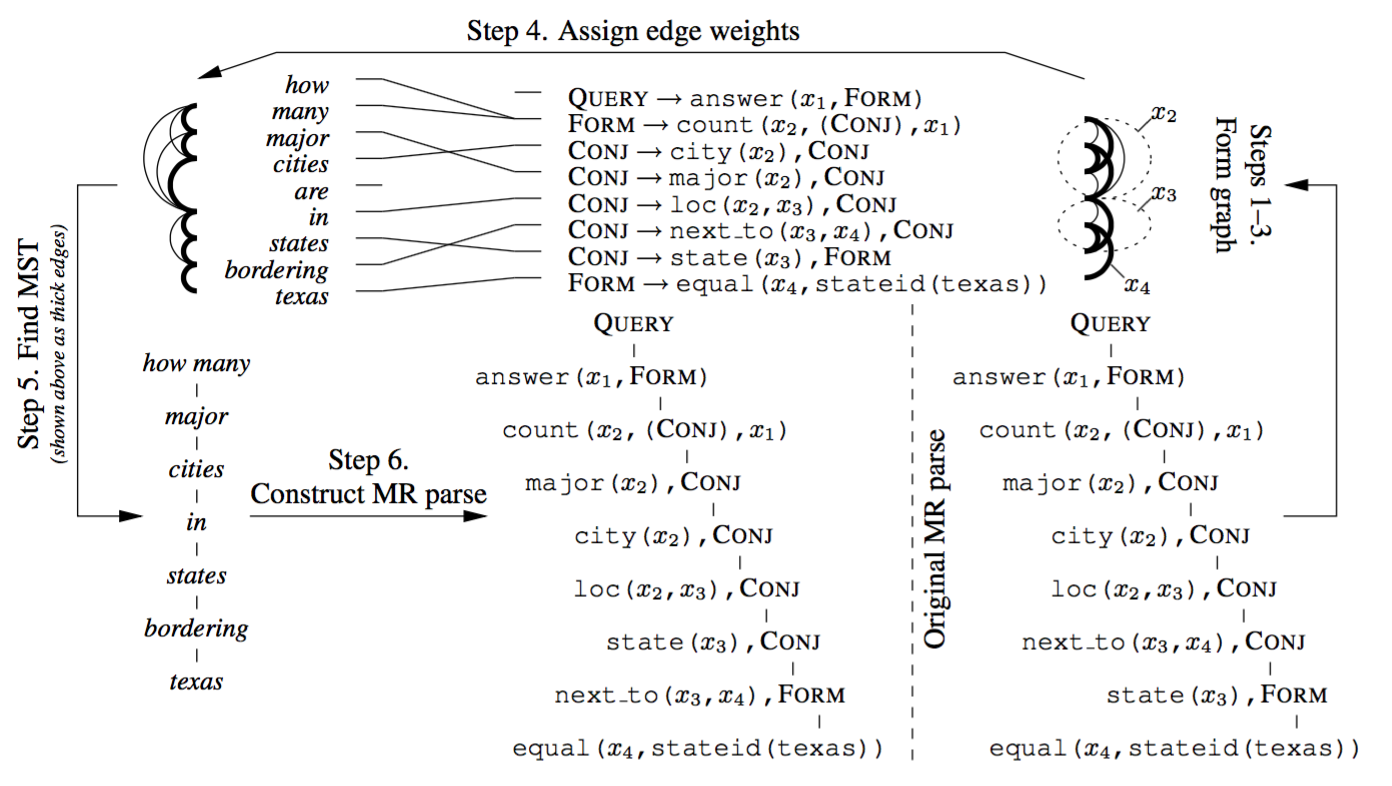
\includegraphics[width=12cm,height=6cm]{img/nl-ml-isomorphism.png}
    \end{center}
\end{frame}

\begin{frame}
    \frametitle{Data Recombination (Jia and Liang, 2016)}

    \only<1> {
        Fit a new model in SCFG using 3 kinds of policies.
        Then draw training examples from it.

        \begin{center}
            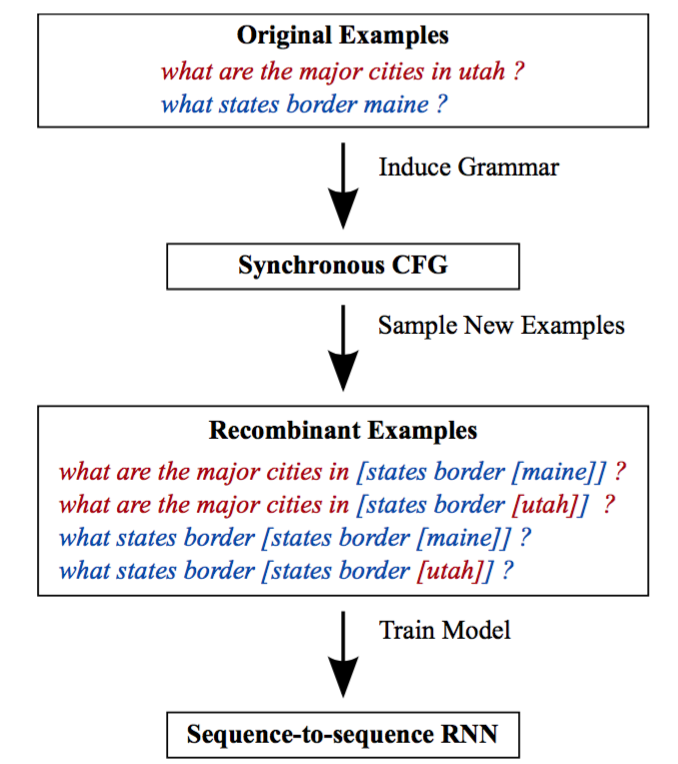
\includegraphics[width=5cm,height=6cm]{img/data-recombinant-system.png}
        \end{center}
    }
    \only<2> {
        \begin{center}
            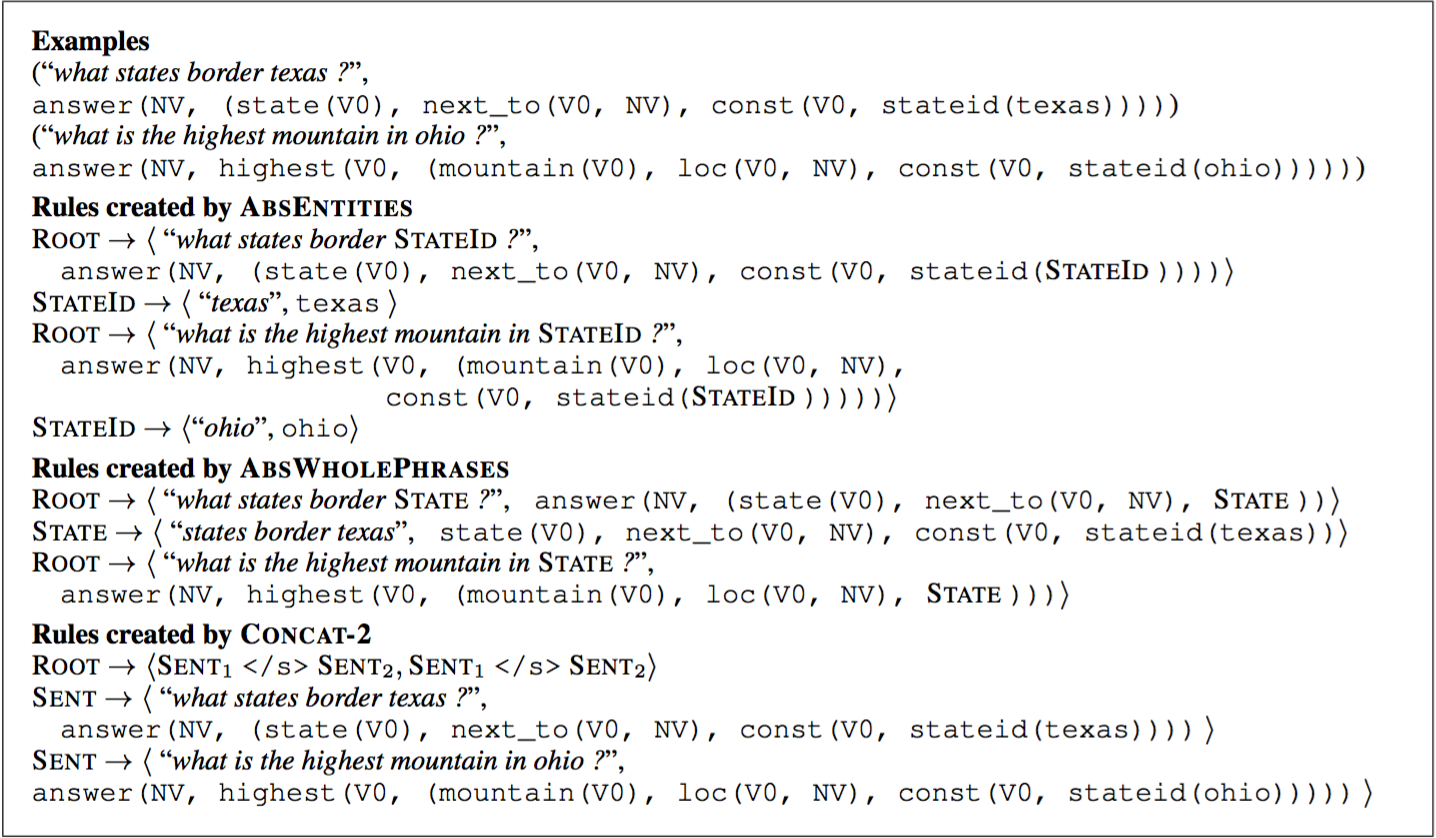
\includegraphics[width=12cm,height=7cm]{img/data-recombinant-example.png}
        \end{center}
    }
\end{frame}

\begin{frame}
    \frametitle{Generative Models}

    \only<1> {
        Hybrid Tree (Lu et al., 2008)

        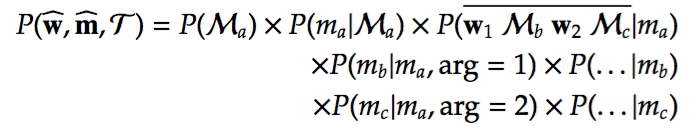
\includegraphics[width=7cm,height=1.3cm]{img/hybrid-tree-model.png}

        \begin{columns}
            \column{0.5\textwidth}

            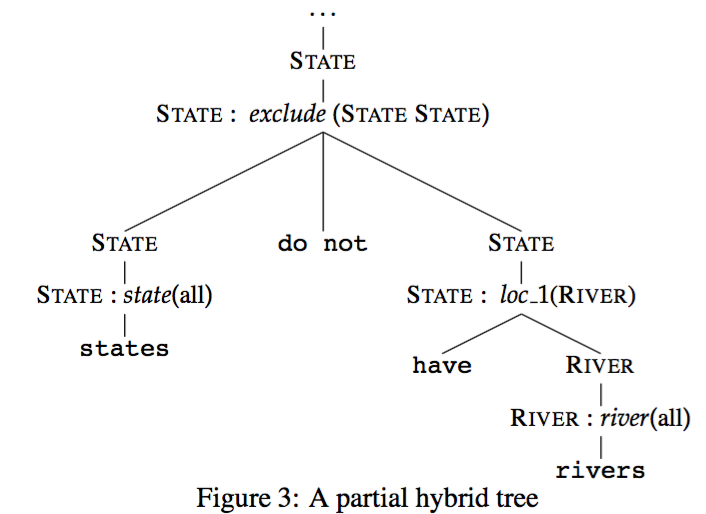
\includegraphics[width=7cm,height=5cm]{img/hybrid-tree-sample.png}
            \column{0.5\textwidth}
            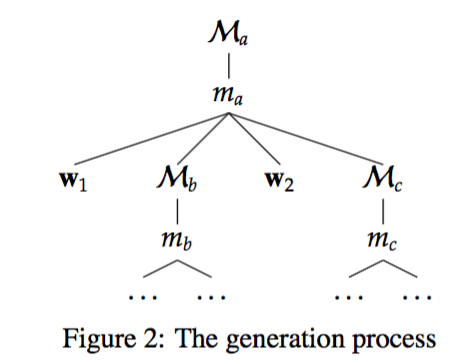
\includegraphics[width=4.6cm,height=3.6cm]{img/hybrid-tree-generation.png}
        \end{columns}
    }

    \only<2> {
        Learning with Less Supervision (Liang et al., 2009)

        Given a World State paired with several sentences.
        \begin{center}
            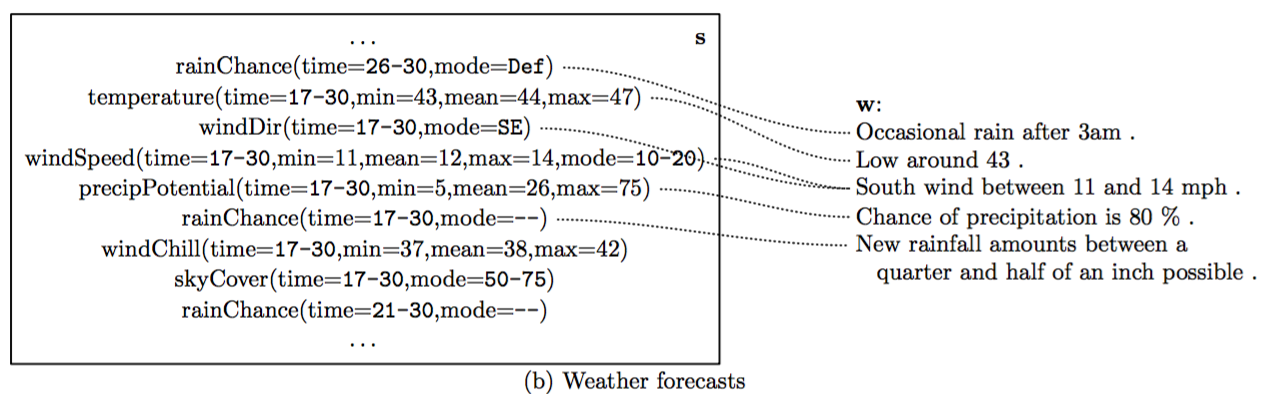
\includegraphics[width=11cm,height=3.0cm]{img/weather-report.png}
        \end{center}
        \[
            p(r, f, c, w \mid s) = p(r \mid s)p(f \mid r)p(c, w \mid r, f, s)
        \]
        \begin{center}
            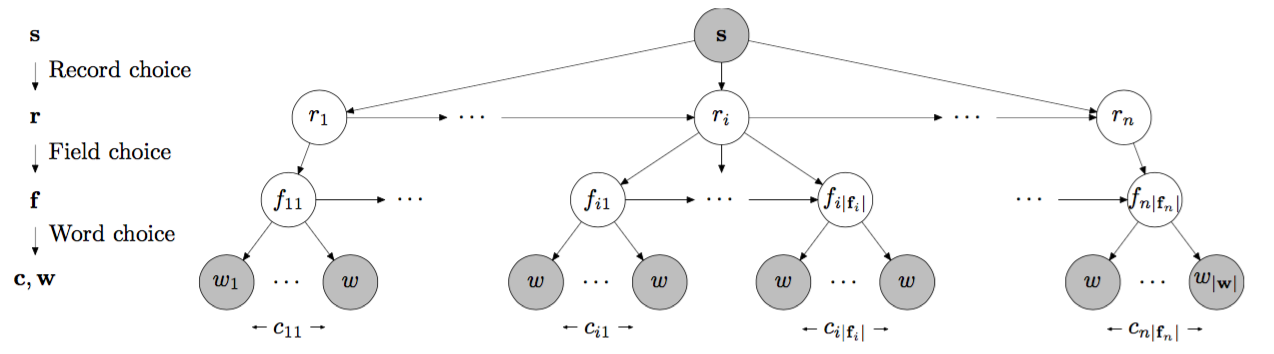
\includegraphics[width=11cm,height=2.7cm]{img/world-state-model.png}
        \end{center}
    }

\end{frame}

\subsection{Semantic Parsing from Syntactic Parses}

\begin{frame}
    \frametitle{Using an Syntactic Parse(Ge and Mooney, 2009)}
    \only<1> {
        Parser Components:
        \begin{itemize}
            \item an existing syntactic parser
            \item a learned lexicon from words to predicates
            \item a learned set of composition rules
        \end{itemize}

        Assumption: unambiguous CFG of LF is known
        \begin{center}
            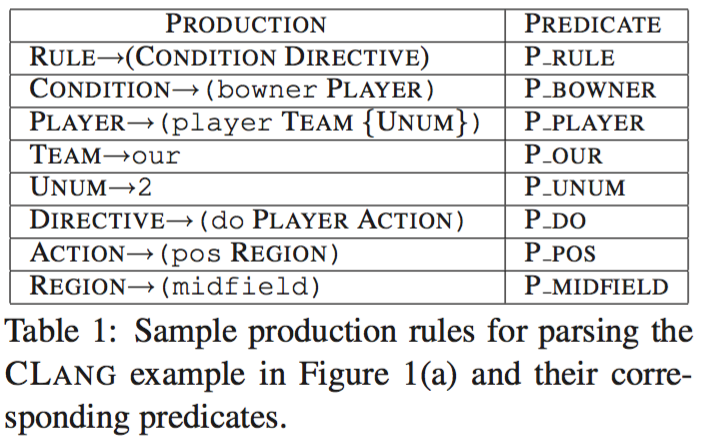
\includegraphics[width=7cm,height=4cm]{img/robocup-mr-grammar.png}
        \end{center}
    }

    \only<2> {
        Parse from bottom-up:
        \begin{center}
            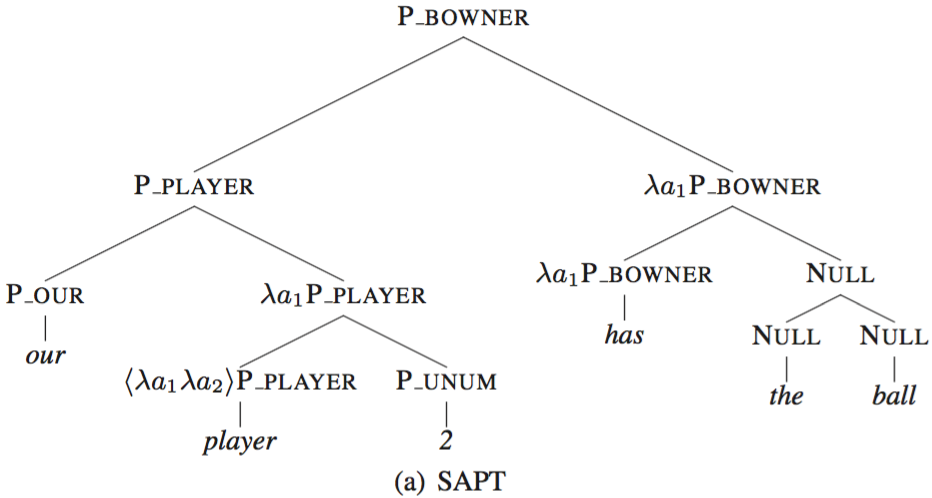
\includegraphics[width=6cm,height=5cm]{img/sapt-parse-01.png}
            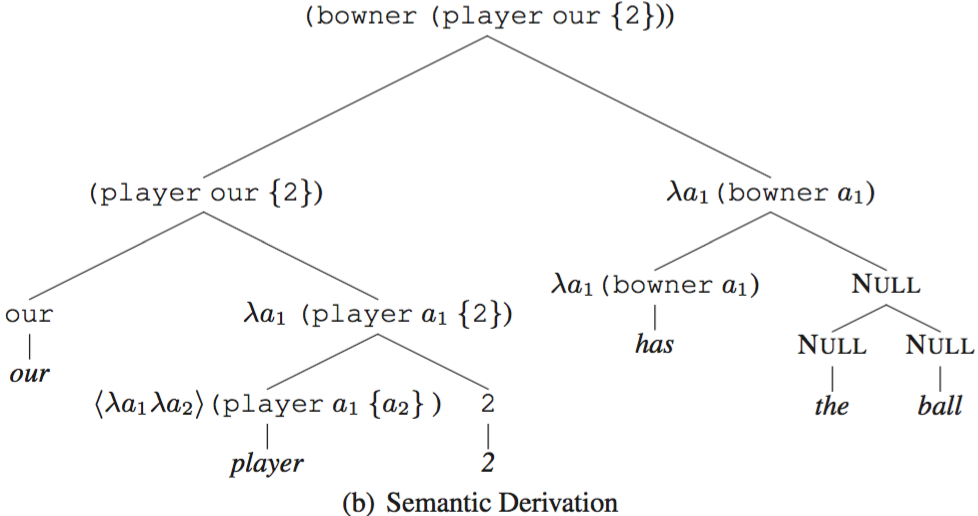
\includegraphics[width=6cm,height=5cm]{img/sapt-parse-02.png}
        \end{center}
    }

    \only<3> {
        Not all semantic sub-tree strictly follows the syntactic derivation.
        Introduce macro-predicates when children MRs can't combine.
        \begin{itemize}
            \item become as an argument if the child MR is complete
            \item otherwise become as part of the predicate
        \end{itemize}

        \begin{center}
            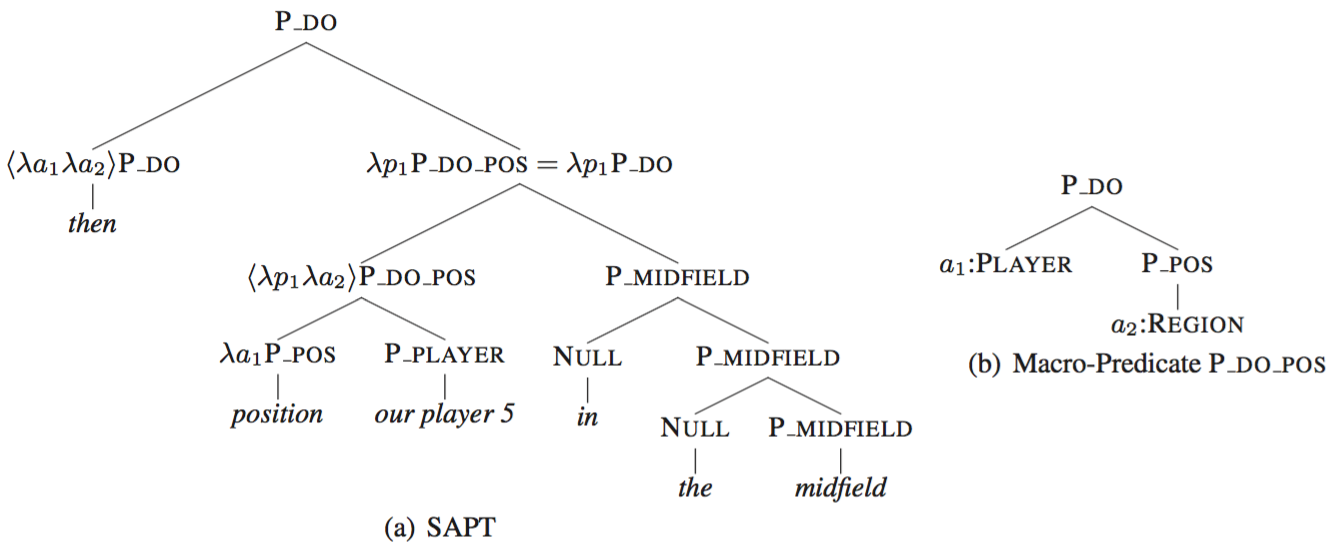
\includegraphics[width=12cm,height=5cm]{img/sapt-parse-macro-predicate.png}
        \end{center}
    }
\end{frame}

\begin{frame}
    \frametitle{Using an Syntactic Parse(Ge and Mooney, 2009)}
    Learning:
    \begin{itemize}
        \item lexicon is learned with GIZA++ (like Wong and Mooney, 2006)
            \begin{itemize}
                \item if a predicate is not aligned to any word, the predicate is inferred
                    and just bound to their values in MR
                \item if a predicate is aligned to several word, split it to several alignments
            \end{itemize}\pause
        \item composition rules is learned in the form $\Lambda_1.P_1 + \Lambda_2.P_2
            \Rightarrow \{\Lambda_p.P_p,R\}$
            \[
                \langle \lambda a_1\lambda a_2\rangle . P\_PLAYER + P\_UNUM \Rightarrow
                \{\lambda a_1.P\_PLAYER, a_2=c_2\}
            \]
        \item disambiguation model: max-ent with L-BFGS
            \[
                \Pr(D\mid S,T;\bar\theta)=\frac{\exp\sum_i\theta_if_i(D)}{Z(S,T)}
            \]
    \end{itemize}
\end{frame}

\begin{frame}
    \frametitle{Transforming Dep. Parse (Reddy et al., 2016)}
    Parsing:
    \only<1> {
        \begin{itemize}
            \item binarize dep parse to S-expr.
            \item substitution symbols with $\lambda$-expr
            \item hierarchical composition(beta-reduction)
        \end{itemize}

        \begin{center}
            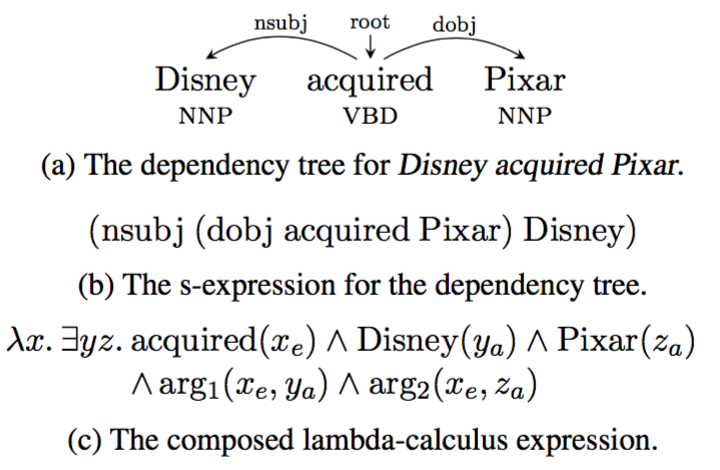
\includegraphics[width=7cm,height=4.5cm]{img/reddy-parse-dep.png}
        \end{center}
    }

    \only<2> {
        Follow Reddy et al. 2014 to transform to grounded graph.

        New operators to deal with mismatch between dep and semantic parse:
        \begin{itemize}
            \item CONTRACT: merge some nodes and edges into a single node
            \item EXPAND: add edges for some disjoint nodes (errors in depparse)
        \end{itemize}

        \begin{center}
            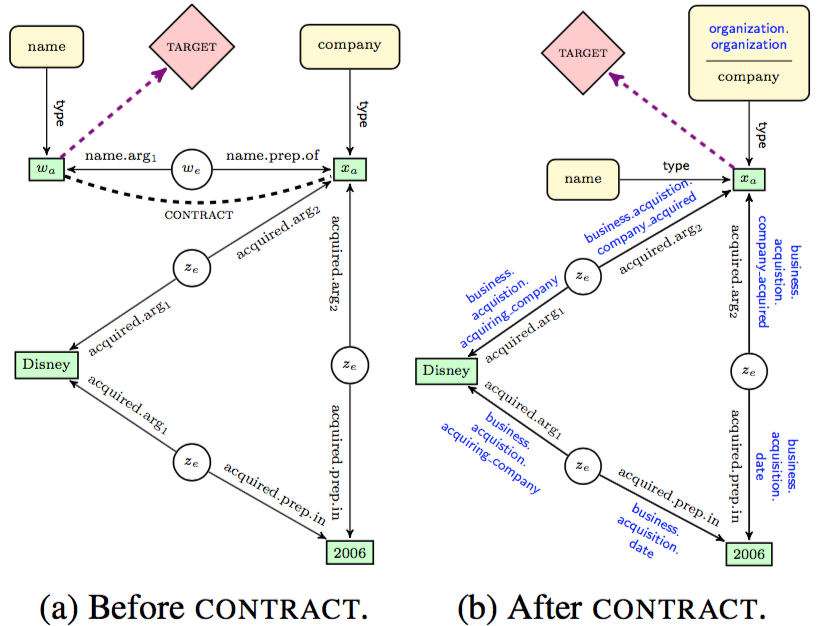
\includegraphics[width=5.3cm,height=4cm]{img/contract-op.png}
        \end{center}
    }
\end{frame}

\begin{frame}
    \frametitle{Other works for SynParse to SemParse}

    \begin{itemize}
        \item Incremental Parser for AMR (Damonte et al. 2016)

            A greedy transition-based parser for AMR, inspired by former work of
            transition-based syntactic parser ArcEager (Nivre 2004, 2008),
            using an existing dep-parser.

        \item Imitation learning for AMR(Goodman et al., 2016)

            A transition-based parser with imitation learning, extended by techniques
            like \emph{noise reduction} and \emph{targeted exploration},
            using an existing dep-parser.

    \end{itemize}
\end{frame}

\subsection{Weak and Unsupervised Parser}
\begin{frame}
    \frametitle{SP from World's Response(Clarke et al., 2010)}
    \only<1> {
        Parsing: $ \hat z = F_w(x)={\arg\max}_{y\in Y,z\in Z}w^T\Phi(x,y,z) $

        Learning:
        \begin{columns}
            \column{0.5\textwidth}
            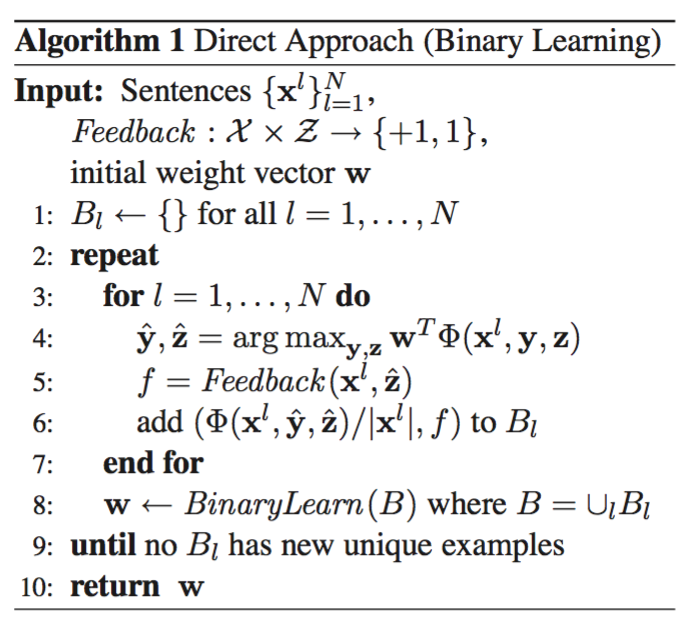
\includegraphics[width=6cm,height=6cm]{img/response-learning-direct.png}
            \column{0.5\textwidth}
            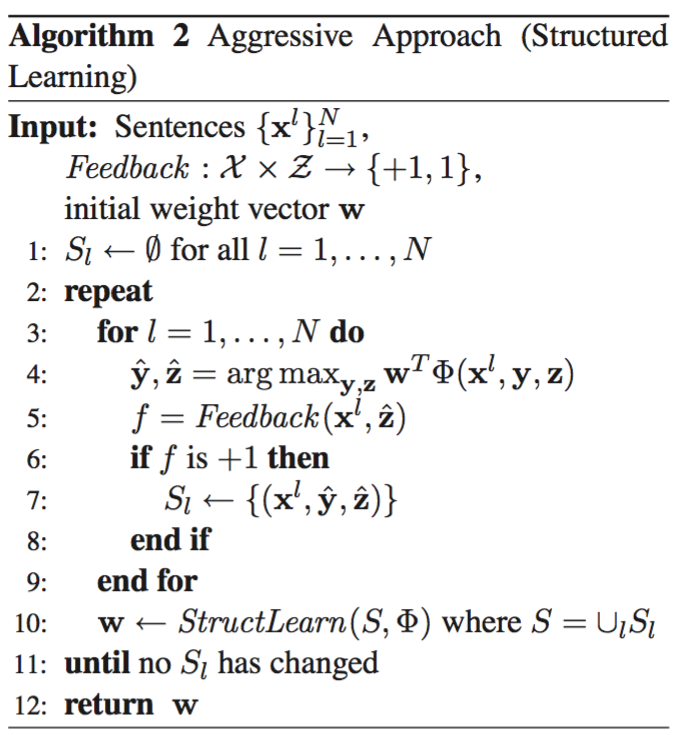
\includegraphics[width=6cm,height=6cm]{img/response-learning-aggressive.png}
        \end{columns}
    }
    
    \only<2-> {
        Parsing: In order to adapt to unseen inputs, consider the entire meaning space
        instead of rule extraction from training data.
        \begin{align*}
            F_w(x)
            &={\arg\max}_{y,z}w^T\Phi(x,y,z) \\
            &={\arg\max}_{\alpha,\beta}\sum_{c\in X}\sum_{s\in D}\alpha_{cs}\cdot w^T\Phi_1
            + \sum_{c,d\in X}\sum_{s,t\in D}\beta_{cs,dt}\cdot w^T\Phi_2
        \end{align*}
    }

    \only<3> {
        \begin{itemize}
            \item $\alpha$: word span $c$ aligned with symbol $s$
            \item $\beta$: word span $d$ aligned with $t$, when $\alpha$ is activated
        \end{itemize}

        such that

        \begin{itemize}
            \item A consituent is associated with 1 symbol
            \item beta(cs,dt) activated iff. alpha(cs) and alpha(dt) activated
            \item beta(cs,dt) activated then s is a function and (s, t) is type-consistent
            \item functional composition is directional and acyclic
        \end{itemize}
    }

    \only<4>{
        Features Used:
        \begin{itemize}

            \item 1st-order: stemmed word match
            \item 1st-order: similarity based on WordNet (Do et al. 2010)
            \item 2nd-order: normalized distance of the head words in c and d
                for beta(cs, dt) on the dependency tree of sentence
            \item 2nd-order: symbol concurrence frequency (regardless of alignments)
        \end{itemize}
    }
\end{frame}

\begin{frame}
    \frametitle{Confidence-driven Unsupervised SP (Goldwasser 2011)}
    \only<1> {
        What is ``confidence-driven unsupervised method'':
        \begin{itemize}
            \item Idea: if a pattern is produced multiple times from non-random model,
                it is likely to be an indication of an underlying phenomenon in the data.

            \item Confidence: Output structures close to the center of statistic mass
                will receive a high confidence score.

            \item Confidence-driven: the model will be significantly improved
                compared with using only prediction score $w^T\Phi(x,y,z)$
        \end{itemize}

        Parsing is the same with Clarke et al. 2010, formulated as an ILP problem.
    }

    \only<2> {
        \begin{columns}
            \column{0.5\textwidth}
            Confidence:

            (1). translation model
            \begin{itemize}

                \item unigram $p(z\mid x)=\prod_{i=1}^{\vert z\vert} p(s_i\mid y(s_i))$
                \item bigram $p(z\mid x)=\prod_{i=1}^{\vert z\vert}
                    p(s_{i-1}(s_i)\mid y(s_{i-1}),y(s_i))$
            \end{itemize}
            (2). structural proportion
            \begin{itemize}
                \item Prop(x, z): proportion of \#pred\_in\_z and \#words\_in\_x
                \item AvProp(S): Average over sets
                \item PropScore(S, (x,z)) = AvProp(S) - Prop(x, z)
            \end{itemize}

            combined: use (2) to filter candidates and (1) to rank items

            \column{0.5\textwidth}
            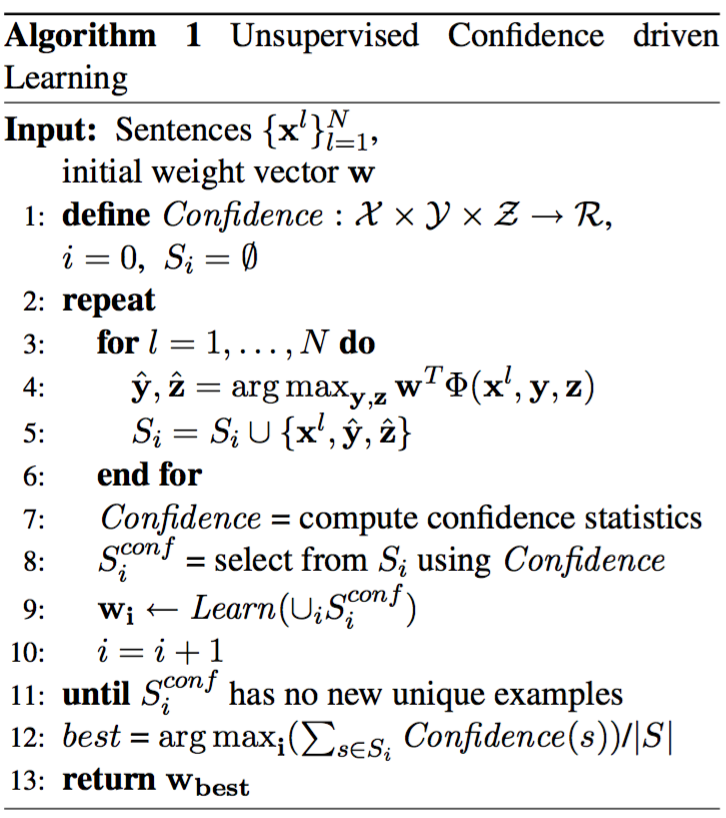
\includegraphics[width=6cm,height=7.5cm]{img/confidence-unsupervised-learning.png}

        \end{columns}
    }
\end{frame}

\begin{frame}
    \frametitle{Grounded Unsupervised SP(Poon, 2013)}

    \only<1> {
        Parsing Idea:
        \begin{itemize}
            \item Annotate states to nodes and edges of a dep-parse
            \item No need to train specific tokens: datetime, numerics, logical op.
        \end{itemize}

        States:
        \begin{itemize}
            \item ``states'' are from DB schema: entity / attribute
            \item complex states are included for mismatching of depparse \& semantic
        \end{itemize}

        Inference:
        \begin{align*}
            z^* &= \arg\max_z P_\theta(d, z) \\
            P_\theta(d,z) &= \frac{1}{Z}\exp\sum_if_i(d,z)\cdot w_i(d,z)
        \end{align*}

        Learning:
        \[
            \theta^* = \arg\max\sum_{d\in D}\log\sum_zP_\theta(d,z)
        \]
    }

    \only<2> {
        \begin{quotation}
            get flight from toronto to san diego stopping in dtw.
        \end{quotation}
        \begin{center}
            \includegraphics[width=8.64cm,height=7.12cm]{img/grounded-unsupervised-parse.png}
        \end{center}
    }
\end{frame}

\begin{frame}
    \frametitle{SP on Freebase and QA}
    \begin{itemize}
        \item Cai and Yates, 2013a, 2013b

            They discuss methods to use an existing parser in new domain.

        \item Berant et al., 2013

            Collect WebQuestions dataset.

        \item Yih et al., 2014
            
            A CNN-based Semantic Model (CNNSM)

        \item Yih et al., 2015

            Staged Query Graph Generation. Find a core inferential chain executed on Freebase.

        \item Pasupat and Liang, 2015

            SP on semi-structured tables. Propose a dataset of tables and adopt a method to 
            convert tables to knowledge graph first.

    \end{itemize}
\end{frame}

\subsection{Paraphrase-driven Parsing}

\begin{frame}
    \frametitle{Paraphrase Comparision}

    \begin{itemize}
        \item (Berant and Liang, 2014): paraphrase independent with KB, using two kinds
            of templates
        \item (Chen et al. 2016): direct paraphrase, using wiktionary
    \end{itemize}

    \begin{center}
        \includegraphics[width=9.48cm,height=5.28cm]{img/paraphrase.png}
    \end{center}
\end{frame}

\begin{frame}
    \frametitle{SP via Paraphrasing(Berant and Liang, 2014)}
    \begin{align*}
        p_\theta(c, z\mid x) &= \frac{1}{Z}\exp(\phi(x,c,z)^T\theta) \\
        \phi(x,c,z)^T\theta &= \phi_{pr}(x,c)^T\theta_{pr} + \phi_{lf}(x,z)^T\phi_{lf}
    \end{align*}

    \begin{center}
        \includegraphics[width=12cm,height=6cm]{img/paraphrase-template.png}
    \end{center}
\end{frame}

\begin{frame}
    \frametitle{Building SP Overnight (Wang et al. 2015)}

    Build an SP for a new Domain (8 published datasets):
    \begin{columns}
        \column{0.5\textwidth}
        \begin{itemize}
            \item Human write a lexicon
            \item The domain-general grammar G induces canonical LFs and utterances
            \item Crowdsourcing to rewrite the awkward utterances into fluent ones
            \item Train a parser using the grammar G, by paraphrasing
        \end{itemize}
        \column{0.5\textwidth}
        \includegraphics[width=6cm,height=7.2cm]{img/sp-overnight.png}
    \end{columns}
\end{frame}

\subsection{Neural Semantic Parsing}
\begin{frame}
    \frametitle{Sequence-based SP (Xiao et al., 2016)}
    \only<1> {
        Vinyals et al. 2015 proved successful to use sequence model on grammar parsing.
        Xiao et al. compaired various sequence forms based on SPO(Wang et al. 2015).
        \begin{itemize}
            \item LF as raw token sequence
            \item DSP (Derivation Sequence Prediction)
            \item DSP-C (Constrained), use grammar to constrain the next rule at testing time
            \item DSP-CL (Constrained Loss), $p'(y_t)$ is normalized only over possible values
            \item CFP (Canonical Form Prediction), predict CF instead which is then parsed to LF
        \end{itemize}
    }
    \only<2> {
        \begin{center}
            \includegraphics[width=12cm,height=4cm]{img/seq-comparison.png}
        \end{center}
    }
\end{frame}

\begin{frame}
    \frametitle{Parsing with Neural Attention(Dong and Lapata, 2016)}
    The Seq2Tree model that also learns latent grammar.
    \begin{center}
        \includegraphics[width=7cm,height=7cm]{img/seq-to-tree.png}
    \end{center}
\end{frame}

\begin{frame}
    \frametitle{Result Comparison}
    \begin{columns}
        \column{0.5\textwidth}
        \includegraphics[width=6cm,height=5cm]{img/result-geoquery.png}
        \column{0.5\textwidth}
        \includegraphics[width=6cm,height=5cm]{img/result-atis.png}
    \end{columns}

    \vspace*{\baselineskip}

    AMR Parsing(F1: 70 Goodman et al. 2016) and WebQuestions(F1: 52.5 Yih et al. 2015)
\end{frame}

\section{Summary}
\begin{frame}
    \frametitle{Summary}
    Problems:
    \begin{itemize}
        \item LF not Well-Formed

            particularly in Neural SP methods, use existing grammar or learned grammar.

        \item Ontology Mismatching

            paraphrasing or other two-phase parsing.

        \item Utterance Explosion

            prefer expansion from meaning space over rule extraction from training data.

        \item Isomorphism between NL(or Syntactic Parse) and Semantic Parse

            add relaxing extensions because NL isn't strict and syn-parse may introduce errors.

    \end{itemize}
\end{frame}

\end{document}
